%=====================================================================
%  ISO8007 MSc Business Analytics Dissertation — Draft Version 2.0
%  Kartikey Sharma | 250559280 | Newcastle University Business School
%  Styling after Yao et al. (2025), Transportation Research Part F,
%  adapted to ISO8007 submission requirements. Monochrome throughout.
%  In-text citation: superscript numeral hyperlinked to the numbered
%  reference index, so that the prose reads continuously.
%=====================================================================
\documentclass[11pt,a4paper]{article}
\usepackage[T1]{fontenc}
\usepackage[utf8]{inputenc}
\usepackage{mathptmx}
\usepackage[scaled=0.90]{helvet}
\usepackage[left=2.4cm,right=2.4cm,top=2.3cm,bottom=2.4cm]{geometry}
\usepackage{microtype}
\usepackage{booktabs}
\usepackage{longtable}
\usepackage{array}
\usepackage{tabularx}
\usepackage{ragged2e}
\usepackage{graphicx}
\usepackage{tikz}
\usetikzlibrary{arrows.meta,positioning,calc,fit,backgrounds}
\usepackage{caption}
\usepackage{enumitem}
\usepackage{setspace}
\usepackage{fancyhdr}
\usepackage{float}
\usepackage{titlesec}
\usepackage{amssymb}
\usepackage{amsmath}
\usepackage[hidelinks]{hyperref}
\numberwithin{figure}{section}
\numberwithin{table}{section}
\setlength{\headheight}{14pt}

\captionsetup[figure]{font=small,labelfont=bf,labelsep=period,justification=justified,
  singlelinecheck=false,name=Fig.}
\captionsetup[table]{font=small,labelfont=bf,labelsep=newline,justification=justified,
  singlelinecheck=false,skip=3pt}

\titleformat{\section}{\normalfont\large\bfseries}{\thesection.}{0.6em}{}
\titleformat{\subsection}{\normalfont\normalsize\bfseries\itshape}{\thesubsection.}{0.6em}{}
\titleformat{\subsubsection}{\normalfont\small\bfseries}{\thesubsubsection.}{0.6em}{}
\titlespacing*{\section}{0pt}{14pt}{6pt}
\titlespacing*{\subsection}{0pt}{11pt}{4pt}
\titlespacing*{\subsubsection}{0pt}{9pt}{3pt}

\setlength{\parindent}{1.2em}
\setlength{\parskip}{0pt}
\onehalfspacing
\renewcommand{\arraystretch}{1.12}

\pagestyle{fancy}
\fancyhf{}
\fancyhead[L]{\footnotesize\itshape K. Sharma}
\fancyhead[R]{\footnotesize\itshape ISO8007 Dissertation, Newcastle University Business School (2026)}
\fancyfoot[C]{\small\thepage}
\renewcommand{\headrulewidth}{0.4pt}

% ---- superscript citation linked to the numbered reference index ----
\newcommand{\cn}[1]{\textsuperscript{\hyperlink{ref#1}{#1}}}
\newcommand{\cnn}[1]{\textsuperscript{#1}}
\newcolumntype{L}[1]{>{\RaggedRight\arraybackslash}p{#1}}
\newcommand{\pend}[2]{%
\begin{center}
\begin{tikzpicture}
\node[draw=black,dashed,line width=0.7pt,rounded corners=2pt,inner sep=8pt,
 text width=0.93\textwidth]{\small\textbf{[TO BE COMPLETED --- #1]}\\[3pt]\small #2};
\end{tikzpicture}
\end{center}}
\newcommand{\nbox}[2]{%
\begin{center}
\begin{tikzpicture}
\node[draw=black,line width=0.7pt,rounded corners=2pt,inner sep=8pt,
 text width=0.93\textwidth]{\small\textbf{#1}\\[3pt]\small #2};
\end{tikzpicture}
\end{center}}

\begin{document}

%=====================================================================
\thispagestyle{empty}
\begin{center}
\rule{\textwidth}{0.8pt}\\[3pt]
\begin{minipage}{0.30\textwidth}\centering
{\footnotesize\sffamily\textbf{NEWCASTLE}\\\textbf{UNIVERSITY}\\\textbf{BUSINESS SCHOOL}}
\end{minipage}%
\begin{minipage}{0.44\textwidth}\centering
{\footnotesize Dissertation submitted in part fulfilment of}\\[2pt]
{\large\itshape MSc Business Analytics}\\[3pt]
{\footnotesize Module ISO8007 \textbullet{} Academic Year 2025/26}
\end{minipage}%
\begin{minipage}{0.24\textwidth}\centering
{\footnotesize Draft Version 2.0\\ 18 August 2026}
\end{minipage}\\[3pt]
\rule{\textwidth}{0.8pt}
\end{center}

\vspace{10pt}
{\setstretch{1.0}\LARGE\bfseries When do dashboards override judgement?\\[3pt]
Decision scenarios, data quality and managerial reliance on\\[3pt] business intelligence dashboards\par}

\vspace{10pt}
{\setstretch{1.0}\large Kartikey Sharma\,\textsuperscript{a,*}\par}
\vspace{3pt}
{\footnotesize\itshape \textsuperscript{a} Newcastle University Business School, 5 Barrack Road, Newcastle upon Tyne NE1 4SE, United Kingdom\par}
\vspace{2pt}
{\footnotesize Student ID: 250559280 \quad\textbullet\quad Supervisor: Dr Xinyue Hao \quad\textbullet\quad Main text: approximately 9,900 words including tables, of a 12,000-word limit\par}

\vspace{12pt}
\rule{\textwidth}{0.5pt}
\vspace{6pt}

\noindent
\begin{minipage}[t]{0.27\textwidth}\setstretch{1.05}
{\footnotesize\sffamily A R T I C L E \; I N F O}\\[2pt]
\rule{\linewidth}{0.4pt}\\[4pt]
{\footnotesize\itshape Keywords:}\\[2pt]
{\footnotesize
Business intelligence dashboards\\
Managerial judgement\\
Over-reliance\\
Data quality\\
Mixed methods\\[8pt]}
{\footnotesize\itshape Draft status:}\\[2pt]
{\footnotesize
Chapters 1--3 complete.\\
Chapter 4 reports the\\
completed documentary\\
strand; the survey and\\
interview strands remain\\
in the field and are marked\\
as pending throughout.\\[8pt]}
{\footnotesize\itshape Citation convention:}\\[2pt]
{\footnotesize
Superscript numerals refer\\
to the numbered reference\\
index and are clickable.}
\end{minipage}\hfill
\begin{minipage}[t]{0.68\textwidth}
{\footnotesize\sffamily A B S T R A C T}\\[2pt]
\rule{\linewidth}{0.4pt}\\[4pt]
{\footnotesize\setstretch{1.06}
\textbf{Purpose.} Business intelligence (BI) dashboards have become the point at which most managerial
decisions now begin. A substantial body of work establishes that managers rely upon such systems, yet
comparatively little is known about the conditions under which that reliance ceases to assist judgement and
begins to displace it. This study therefore asks not whether managers defer to dashboards, but in which
decision scenarios they do so, why, and with what consequence for decision accuracy and creative
exploration.\\[3pt]
\textbf{Design.} An integrated behavioural framework is developed which links dashboard design and visual
framing, the visibility of data-quality defects, and the organisational accountability regime to three
decision outcomes. A pragmatist, critical realist mixed-methods design is adopted across three strands: a
scenario-based decision experiment employing experimental vignette methodology; a structured documentary
analysis of publicly evidenced analytics failures; and semi-structured interviews sampled upon observed
experimental behaviour.\\[3pt]
\textbf{Findings.} The completed documentary strand codes twelve organisational failures against a fixed
extraction frame, drawing exclusively upon regulator enforcement notices, statutory inquiry reports and
royal commission findings across nine sectors and four jurisdictions. Two patterns emerge. Defects that
were silent at the point of use persisted for years, whereas defects that produced any perceptible signal
were recognised within hours or days. More consequentially, in nine of the twelve cases a human challenge
to the system output was in fact raised and was then overridden, ignored or not acted upon.\\[3pt]
\textbf{Originality.} The finding that challenge was raised and suppressed, rather than never raised at
all, obliges a revision of the initial framework. Attentional accounts of automation bias explain why
managers might fail to notice a defect; they do not explain why noticing repeatedly failed to produce
action. The study therefore distinguishes \emph{detection failure} from \emph{authority failure} and
proposes legitimacy asymmetry as the mechanism connecting them. The practical implication is that
governance investment directed at better warnings addresses the wrong constraint.\par}
\end{minipage}

\vspace{8pt}
\rule{\textwidth}{0.5pt}
\vspace{4pt}

\noindent{\footnotesize * Corresponding author. \textit{E-mail address:} k.sharma7@newcastle.ac.uk (K. Sharma).\par}
\noindent{\footnotesize Draft of 18 August 2026; Strand 1 and Strand 3 data collection ongoing.\par}

\vspace{10pt}
\rule{\textwidth}{0.8pt}

\newpage
%---------------------------------------------------------------------
\section*{Acknowledgements}
\addcontentsline{toc}{section}{Acknowledgements}

I am grateful to my supervisor, Dr Xinyue Hao, for guidance on framing the research questions
conditionally rather than assuming the behaviour that this study sets out to examine. I also wish to
thank the examiners of the NBS8062 research proposal, whose comments on the coherence of the conceptual
argument and on the specificity of the secondary data strand shaped the present design in a direct and
material way. Any errors that remain are, of course, entirely my own.

\vspace{6pt}
\section*{Statement on the use of generative artificial intelligence}
\addcontentsline{toc}{section}{Statement on the use of generative AI}

Generative artificial intelligence tools were used to assist with document formatting, the preparation of
figures from coded data, and language editing. All research design decisions, source selection, coding
judgements, analysis and interpretation are my own. Every source cited has been checked against its
primary record and is listed with its access route in the accompanying reference register.

\newpage
\setcounter{tocdepth}{2}
\tableofcontents
\vspace{10pt}
\listoffigures
\vspace{10pt}
\listoftables

\vspace{12pt}
\section*{Abbreviations}
\addcontentsline{toc}{section}{Abbreviations}
\begin{tabular}{@{}p{2.2cm} p{12.5cm}@{}}
BI & Business intelligence \\
CAA & Civil Aviation Authority (United Kingdom) \\
FCA & Financial Conduct Authority (United Kingdom) \\
GDPR & General Data Protection Regulation \\
KPI & Key performance indicator \\
MRS & Market Research Society \\
OCC & Office of the Comptroller of the Currency (United States) \\
OSR & Office for Statistics Regulation (United Kingdom) \\
RQ & Research question \\
SEC & Securities and Exchange Commission (United States) \\
\end{tabular}

\newpage
%=====================================================================
\section{Introduction}
%=====================================================================

\subsection{Background}

Managerial decision-making in the contemporary organisation rarely begins with a blank sheet of paper. It
begins with a screen. Business intelligence dashboards have evolved over two decades from comparatively
passive reporting interfaces into what may reasonably be termed decision infrastructure: they determine
which indicators are placed before the manager, which are aggregated away, which are shaded red, and,
most consequentially, which account of organisational reality proves easiest to defend when the decision
is later questioned.

The literature has been broadly favourable towards these systems, and with good reason. BI and analytics
capabilities are consistently associated with improved decision support and organisational performance,
principally because they integrate dispersed data, visualise performance and embed analysis within routine
managerial work\textsuperscript{\hyperlink{ref14}{14},\hyperlink{ref23}{23},\hyperlink{ref62}{62},\hyperlink{ref69}{69}}. Within operations, logistics and
supply chain management, dashboards support demand monitoring, inventory visibility, transport performance
measurement and disruption response\textsuperscript{\hyperlink{ref31}{31},\hyperlink{ref33}{33},\hyperlink{ref73}{73}}. The benefit is real and
this study does not dispute it.

What is less well understood is the other side of the ledger. A dashboard does not display reality; it
composes it. In selecting indicators, aggregating complexity, assigning colours and ranking priorities, the
interface necessarily renders certain forms of knowledge more visible than others\textsuperscript{\hyperlink{ref51}{51},\hyperlink{ref59}{59},\hyperlink{ref77}{77}}.
This compression is simultaneously the source of the dashboard's value and of its risk. A dashboard may
therefore become a quiet governor of judgement --- polished, auditable and persuasive --- even where the
underlying data happen to be incomplete, delayed or excessively aggregated.

\subsection{The research problem}

The stakes are not hypothetical, and it is worth grounding the problem in the public record before
proceeding to theory. The Post Office Horizon IT Inquiry found that system-generated accounting data was
treated as authoritative over the contrary accounts of several hundred sub-postmasters, with consequences
that were by any measure catastrophic\textsuperscript{\hyperlink{ref54}{54}}. The Royal Commission into the Robodebt Scheme in
Australia documented how a debt-raising system built upon averaged income data reversed the onus of proof
onto citizens, and how internal legal advice questioning its lawfulness was obtained and then set
aside\textsuperscript{\hyperlink{ref56}{56}}. In a different setting entirely, the United Kingdom Civil Aviation Authority's
independent review of the 2023 flight-planning failure at NATS described how an automated system's response
to a single ambiguous input propagated into national disruption, and how escalation to the engineers
capable of diagnosing the fault proved slower than the failure itself\textsuperscript{\hyperlink{ref15}{15}}.

On close reading these are not stories about badly designed software. They are stories about what happens
when a system output becomes more institutionally credible than a human objection. That distinction is the
point of departure for this study.

The difficulty is that the literature has largely established \emph{that} reliance upon analytical outputs
occurs, without specifying with precision \emph{under which decision conditions} such reliance becomes
hazardous, and \emph{why} organisational context makes it rational for the individual manager to defer even
where deference proves costly for the organisation. Indeed, the evidence is genuinely contested.
Individuals may be markedly averse to algorithmic advice after observing it err\textsuperscript{\hyperlink{ref20}{20}}, and yet in
other conditions display a clear preference for algorithmic over human judgement\textsuperscript{\hyperlink{ref40}{40}}. Systematic
reviews conclude that reliance is best understood as condition-dependent rather than as a stable individual
trait\textsuperscript{\hyperlink{ref13}{13},\hyperlink{ref42}{42}}. If that conclusion is sound, then the useful research question must
itself be conditional.

\subsection{Aim and objectives}

The aim of this study is to identify the decision conditions under which managers prioritise BI dashboard
outputs over intuition and contextual judgement, to explain why such prioritisation occurs and becomes
entrenched, and to assess its consequences for decision accuracy and for the generation of alternative
courses of action.

The objectives are as follows.

\begin{enumerate}[leftmargin=*,itemsep=2pt,topsep=4pt]
\item To establish experimentally how decision risk, the visibility of data-quality signals and
accountability framing jointly affect the probability that a manager follows a dashboard output which
conflicts with contextual evidence.
\item To measure whether dashboard deference is associated with reduced generation of alternative courses
of action.
\item To characterise, from publicly evidenced organisational failures, how analytics and reporting errors
persist undetected, and whether human challenge was raised, escalated or overridden.
\item To explain, through professional accounts, why dashboard outputs acquire greater institutional
legitimacy than contextual judgement.
\item To develop a governance framework for preserving analytical rigour whilst protecting human challenge.
\end{enumerate}

\subsection{Research questions}

\nbox{Research questions}{%
\textbf{RQ1 (when, and with what consequence).} In what decision scenarios do managers prioritise BI
dashboard outputs over intuition and contextual judgement, and how does that prioritisation relate to
decision accuracy and to the generation of alternative courses of action?\\[3pt]
\hspace*{10pt}\textbf{RQ1a} How do decision risk, data-quality signal visibility, accountability framing and
metric salience affect the likelihood of following a dashboard output which conflicts with contextual
evidence?\\
\hspace*{10pt}\textbf{RQ1b} Is dashboard deference associated with narrower generation of alternative
actions, after controlling for experience and sector?\\[5pt]
\textbf{RQ2 (why).} Why do managers prioritise dashboard outputs in those scenarios, and what organisational
conditions entrench or interrupt that prioritisation?\\[3pt]
\hspace*{10pt}\textbf{RQ2a} What reasons do professionals offer --- perceived objectivity, auditability,
time pressure, professional defensibility --- for following or challenging dashboard outputs?\\
\hspace*{10pt}\textbf{RQ2b} What governance, cultural or role conditions make challenge possible?}

\subsection{Scope and boundaries}

Three boundaries should be stated at the outset, since a study of this length cannot address everything
that the topic invites.

Firstly, the unit of analysis is the \emph{individual decision episode} rather than the organisation or the
system. The study does not evaluate dashboard software, nor does it assess the return on analytics
investment. Secondly, the study concerns BI dashboards and organisational analytics rather than generative
artificial intelligence. Recent work on reliance upon artificial intelligence is drawn upon where the
mechanism is shared\textsuperscript{\hyperlink{ref12}{12},\hyperlink{ref72}{72}}, but generative systems introduce questions of
fluency and fabrication that lie outside the present design. Thirdly, the study is concerned with
professional decision-making in commercial and public sector settings in which dashboards are used at least
weekly; it makes no claim about consumer or clinical contexts, where the automation bias literature is
considerably better developed\textsuperscript{\hyperlink{ref29}{29},\hyperlink{ref41}{41}}.

\subsection{Contribution}

The intended contribution is a condition-specific account of dashboard reliance. Rather than asking whether
analytics adds value --- a question the literature has largely answered affirmatively --- the study asks
when analytics creates fragility, and triangulates the answer across three distinct evidential bases:
experimental behaviour under controlled variation, documented organisational failure, and the explanations
offered by practising professionals. As Section~5 sets out, the documentary strand has already required a
substantive revision of the initial framework, which is itself part of the contribution.

\subsection{Structure}

Section~2 reviews the literature as a single connected argument, appraises the quality of the evidence
critically, and states the research gap. Section~3 sets out the philosophical position, the design
alternatives considered and rejected, the three empirical strands, the quality criteria and the ethical
safeguards. Section~4 presents the findings, beginning with the completed documentary strand. Section~5
discusses these against the conceptual framework and proposes a revision to it. Section~6 concludes,
proposes a governance framework, and identifies limitations and further research.

%=====================================================================
\section{Literature review}
%=====================================================================

\subsection{Scope and method of the review}

The review was conducted through structured searches of Scopus, Web of Science and Business Source Premier,
supplemented by forward and backward citation chaining from the five most central papers. Five search
strings were used, combining terms for BI dashboards, algorithmic reliance and automation bias, data and
information quality, creativity and option generation, and the unintended consequences of performance
management. Retrieval was restricted to peer-reviewed journal articles published in English, with a
principal window of 2015 to 2026 for the reliance and dashboard literatures and no lower bound for
foundational works retained by hand. Conference proceedings were admitted only where the venue is the
principal outlet for the field, which applies to human-computer interaction research. Grey literature was
admitted only where it constitutes primary evidence for the documentary strand, in which case the
admissibility rules of Section~3.6 apply.

The review is organised as one continuous argument rather than as a series of parallel summaries, since the
contribution rests upon the connections between these literatures rather than upon any of them
individually. The argument proceeds in five linked steps, and Section~2.7 then appraises the quality of the
evidence supporting each.

\subsection{Bounded rationality and the demand for simplified cues}

Managers satisfice. Simon's behavioural model of rational choice establishes that decision-makers operate
under limits of information, time and cognitive capacity, and consequently adopt simplifying strategies
that are adequate rather than optimal\textsuperscript{\hyperlink{ref65}{65}}. Kahneman subsequently distinguished fast, associative
processing from slow and effortful processing, noting that expertise yields reliable pattern recognition
only in environments supplying consistent feedback\textsuperscript{\hyperlink{ref34}{34}}.

A dashboard is an unusually attractive satisficing device. It converts a high-dimensional problem into a
small number of pre-evaluated signals at almost negligible cognitive cost. Consider, by way of
illustration, a regional operations manager deciding on a Monday morning whether to authorise expedited
freight for a product line. The complete problem involves supplier reliability, port congestion, contract
terms, seasonality and the working-capital position. The dashboard offers a single amber indicator reading
``service level at risk''. The manager is not being lazy in attending to it; she is behaving as Simon would
predict.

The implication is directional and worth stating carefully. Bounded rationality does not predict that
managers will believe dashboards to be true. It predicts that under time pressure they will \emph{cease
searching} once a sufficiently authoritative-looking cue becomes available. The behavioural question is
therefore not one of belief but of search termination --- and search termination is what dashboard design
governs.

\subsection{From cognition to interface: design, salience and confidence}

If bounded rationality creates the demand for simplified cues, dashboard design determines the supply.
Research on performance dashboards shows that layout, metric selection, update frequency and visual
encoding shape interpretation and use\textsuperscript{\hyperlink{ref51}{51},\hyperlink{ref77}{77}}. Sarikaya and colleagues demonstrated,
through analysis of a large corpus of real dashboards, that the term covers a wide design space whose
variants afford sharply different behaviours, ranging from open exploration to compliance-oriented
monitoring\textsuperscript{\hyperlink{ref59}{59}}; Bach and colleagues have since catalogued the recurring patterns through which
dashboards structure attention\textsuperscript{\hyperlink{ref7}{7}}. Underpinning this, foundational visualisation research explains
the mechanism: graphical perception and visual encoding determine what users notice and how accurately they
read quantitative information\textsuperscript{\hyperlink{ref16}{16},\hyperlink{ref70}{70},\hyperlink{ref75}{75}}.

The transition from cognition to interface is therefore causal rather than merely thematic. Where Simon
explains why a manager will accept a simplified cue, visualisation research explains which cue that will be
--- the one possessing highest visual salience --- and how confident the manager will feel whilst accepting
it. Confidence is the pivotal variable. A red-amber-green indicator does not merely summarise a position;
it signals that the interpretive work has already been completed by somebody else.

The behavioural consequence is documented in the automation-bias literature. Individuals misuse automation
by accepting system outputs too readily\textsuperscript{\hyperlink{ref50}{50}}, and automated cues encourage acceptance even
where contradictory evidence is available\textsuperscript{\hyperlink{ref45}{45},\hyperlink{ref66}{66}}. Parasuraman and Manzey integrated
these findings through attention, arguing that reliance reduces the attentional sampling of raw
evidence\textsuperscript{\hyperlink{ref49}{49}}. Systematic reviews in clinical settings confirm both the frequency of the
effect and its sensitivity to verification cost: the harder it is to check the system, the more readily it
is trusted\textsuperscript{\hyperlink{ref29}{29},\hyperlink{ref41}{41}}.

The contemporary literature nonetheless rejects any simple account in which people merely over-trust
machines. Observing an algorithm err produces disproportionate abandonment\textsuperscript{\hyperlink{ref20}{20}}, whilst other
tasks reveal a general preference for algorithmic over human judgement\textsuperscript{\hyperlink{ref40}{40}}. The apparent
contradiction is resolved by reviews concluding that reliance varies with task type, perceived expertise,
error visibility and retained control\textsuperscript{\hyperlink{ref13}{13},\hyperlink{ref42}{42}}. This is the single most important
justification for the conditional framing of RQ1. Studies of artificial intelligence-assisted decision
making extend the point usefully: over-reliance can be reduced by cognitive forcing functions that raise
the cost of uncritical acceptance\textsuperscript{\hyperlink{ref12}{12}}, and explanations reduce over-reliance only where engaging
with the explanation is less effortful than performing the task oneself\textsuperscript{\hyperlink{ref72}{72}}. Reliance would
appear, then, to be an engineering and governance variable rather than a personality trait.

\subsection{Why data quality is a behavioural problem}

Data quality is conventionally defined across dimensions of accuracy, timeliness, completeness, consistency
and relevance\textsuperscript{\hyperlink{ref74}{74}}, and must be assessed in context, since information that is technically available
may be unfit for a particular decision task\textsuperscript{\hyperlink{ref52}{52},\hyperlink{ref67}{67}}. Poor data quality imposes
substantial organisational cost\textsuperscript{\hyperlink{ref55}{55}}, and remains a managerial rather than a purely technical
responsibility that most organisations systematically under-measure\textsuperscript{\hyperlink{ref46}{46}}. Decision quality in
big-data settings depends upon the whole decision chain rather than upon data alone\textsuperscript{\hyperlink{ref32}{32}}, and
upstream data problems compound invisibly into downstream cascades in high-stakes
systems\textsuperscript{\hyperlink{ref58}{58}}.

The behavioural argument advanced here, and largely absent from that literature, is that data-quality
defects are dangerous \emph{because they are visually silent}. An outdated metric, a partial extract or an
inconsistent definition renders on screen exactly as cleanly as a valid one. There is no perceptual
difference between a trustworthy green indicator and an untrustworthy one.

A concrete illustration may help. Suppose a demand dashboard draws upon a nightly extract which, owing to a
change in an upstream schema, has silently stopped ingesting one of fourteen regional feeds. The dashboard
will not display an error. It will display a slightly lower national demand figure, in the same typeface,
the same colour and the same position as always. The manager reviewing it experiences no cue that anything
is amiss. Contrast this with a dashboard displaying a small banner reading ``data as at 12 August; 1 of 14
feeds not received''. The underlying defect is identical; the behavioural situation is entirely different.

Combining this with the preceding step produces the study's core prediction: the harm arising from poor
data quality is not proportional to the magnitude of the error but to the confidence with which the error
is displayed. This motivates the experimental manipulation of signal visibility described in Section~3.5.
Where the defect is signalled, verification cost falls and challenge should rise; where hidden, the manager
possesses no cue capable of triggering the slower processing that Kahneman describes.

\subsection{Legitimacy asymmetry}

Individual cognition alone cannot explain persistent deference, for the straightforward reason that
experienced managers frequently do suspect that a dashboard is wrong. Something further is required, and
that something is institutional.

Decision support systems are not neutral tools; they participate in organisational knowing and reshape
decision routines\textsuperscript{\hyperlink{ref4}{4},\hyperlink{ref63}{63}}. Performance measurement systems generate well-documented
unintended consequences, amongst them gaming, tunnel vision and the displacement of judgement by measurable
proxies\textsuperscript{\hyperlink{ref28}{28}}. Espeland and Sauder demonstrated reactivity: once a measure becomes publicly
consequential, organisations reorganise around it, and the measure begins to constitute the reality it
claims merely to describe\textsuperscript{\hyperlink{ref24}{24}}.

From these strands the study derives its central organisational construct, \emph{legitimacy asymmetry}. The
argument may be stated simply. A dashboard-based decision is standardised, visual, auditable and defensible
after the event. A judgement-based objection is contextual, tacit and difficult to document. When outcomes
are subsequently reviewed, ``the dashboard showed green'' constitutes a complete defence, whereas ``it did
not feel right to me'' does not. The asymmetry is not one of accuracy but of \emph{defensibility}.

Supporting evidence is available from adjacent literatures. Algorithmic systems function as instruments of
organisational control rather than merely as sources of information\textsuperscript{\hyperlink{ref35}{35}}, and professionals
disengage critical judgement where system opacity renders challenge professionally risky\textsuperscript{\hyperlink{ref38}{38}}.
The resulting design problem may be framed as one of allocating decision authority between humans and
systems\textsuperscript{\hyperlink{ref64}{64}}.

Legitimacy asymmetry thus explains what cognition alone cannot: that deference may be individually rational
even where organisationally costly. It also generates a testable prediction --- that framing a decision as
auditable should raise deference independently of the underlying data --- examined as H2 below.

\subsection{Option-set narrowing and creative exploration}

Creativity is treated here not as an artistic quality but as a decision-quality outcome, namely the
capacity to generate alternative interpretations and courses of action under uncertainty. Evaluation
pressure, control and rigid performance systems reduce creative output\textsuperscript{\hyperlink{ref2}{2}}; organisational
creativity resides in the interaction of individual, group and contextual conditions\textsuperscript{\hyperlink{ref76}{76}}; and
creativity is defined through the joint criteria of originality and effectiveness\textsuperscript{\hyperlink{ref57}{57}}. The
state-of-the-science synthesis confirms the contextual contingency of creative behaviour\textsuperscript{\hyperlink{ref3}{3}}.

The specific mechanism proposed is \emph{option-set narrowing}. A dashboard does not forbid alternatives.
It renders certain options visible and pre-quantified whilst leaving others unmeasured and considerably
harder to argue for. Under time pressure and accountability, the unmeasured option is not so much rejected
as never seriously formulated. Returning to the freight example: expediting shipment appears on the
dashboard with a cost attached, whereas renegotiating the delivery window with the customer does not appear
at all. The second option may well be superior, but the manager would have to construct the case from
scratch and then defend a decision for which no system evidence exists.

Two contemporary findings make this an empirical question rather than an assumption. Artificial
intelligence capability has been found positively associated with organisational creativity, indicating
that analytics may expand exploration\textsuperscript{\hyperlink{ref44}{44}}. Conversely, generative artificial intelligence has
been found to raise individual creative output whilst reducing the collective diversity of ideas
produced\textsuperscript{\hyperlink{ref21}{21}}. The tension is conditional, and this study operationalises it by measuring the
breadth of alternatives a manager generates alongside deference.

\subsection{Critical appraisal of the evidence base}

Master's-level engagement requires more than an accurate summary of what these literatures claim; it
requires an assessment of how far the claims can bear the weight placed upon them. Four weaknesses in the
evidence base deserve explicit statement, since each has shaped the design that follows.

\emph{Ecological validity in the reliance literature.} The foundational reliance experiments are conducted
largely with student samples on generic forecasting or estimation tasks\textsuperscript{\hyperlink{ref20}{20},\hyperlink{ref40}{40}}. Such
tasks strip out precisely the variable this study regards as decisive, namely organisational
accountability. A student predicting an airline passenger's rank faces no career consequence for being
wrong, whereas a manager overruling a dashboard does. Findings from those settings should therefore be
treated as establishing that reliance is malleable, not as establishing its magnitude in professional
contexts. This study responds by recruiting practising professionals and by manipulating accountability
directly.

\emph{Domain concentration in the automation-bias literature.} The most rigorous evidence on automation
bias comes from aviation and clinical decision support\textsuperscript{\hyperlink{ref29}{29},\hyperlink{ref41}{41},\hyperlink{ref45}{45}}. These are
high-reliability domains with formal escalation procedures, mandatory logging and, frequently, a second
qualified operator. Managerial dashboard use has none of these features. It is therefore an open question
whether findings transfer, and the direction of the bias is not obvious: managers may challenge more
readily because no formal procedure constrains them, or less readily because no procedure protects them.

\emph{Measurement, not behaviour, in the data-quality literature.} The data-quality tradition is unusually
strong on conceptualisation and unusually weak on consequence. The canonical dimensional
frameworks\textsuperscript{\hyperlink{ref52}{52},\hyperlink{ref67}{67},\hyperlink{ref74}{74}} were developed to support assessment and improvement
programmes, not to predict what a decision-maker will do when a dimension degrades. Even the more recent
managerial work reports the extent of under-measurement rather than the behavioural response to
it\textsuperscript{\hyperlink{ref46}{46}}. This is a genuine gap rather than a criticism of those authors' intent, and it is the gap
that hypothesis H1 targets.

\emph{Correlational designs in the analytics-value literature.} Studies linking analytics capability to
firm performance rely overwhelmingly upon cross-sectional survey data with self-reported measures of both
capability and performance\textsuperscript{\hyperlink{ref31}{31},\hyperlink{ref44}{44},\hyperlink{ref73}{73}}. Such designs are exposed to
common method bias and to reverse causality, since successful firms can afford better
analytics\textsuperscript{\hyperlink{ref53}{53}}. The positive case for BI summarised in Section~2.1 is therefore weaker than its
volume suggests, which is a point rarely made in dissertations on this topic and one that strengthens
rather than weakens the rationale for the present study.

Taken together, these four weaknesses point in a single direction. The literature is strong on mechanism
and weak on organisational condition. A design that varies condition explicitly, in a professional
population, and triangulates against documented organisational outcomes, is therefore a defensible
response rather than merely an ambitious one.

\subsection{Synthesis, research gap and conceptual framework}

The literature establishes each link separately. Bounded rationality creates demand for simplified cues;
visual design determines salience and confidence; data-quality defects are invisible at the point of use;
accountability regimes render system-based decisions more defensible; and organisational systems constrain
creative exploration. What has not been attempted is examination of these links as one causal chain, under
controlled decision conditions, in realistic professional settings. More specifically: reliance research is
dominated by generic algorithmic-advice tasks rather than by dashboards embedded in accountability
structures; data-quality research measures dimensions and cost but seldom the behavioural response to a
hidden as against a signalled defect; dashboard design research addresses comprehension rather than
decision error under conflicting evidence; and creativity is almost never measured as a co-outcome
alongside accuracy and reliance in the same study.

\nbox{The gap addressed by this study}{%
There exists no integrated empirical account specifying the decision conditions under which BI dashboard
reliance shifts from being a decision \emph{aid} to being a decision \emph{risk}, nor explaining why
organisational context sustains that shift once it has occurred.}

\begin{figure}[H]
\centering
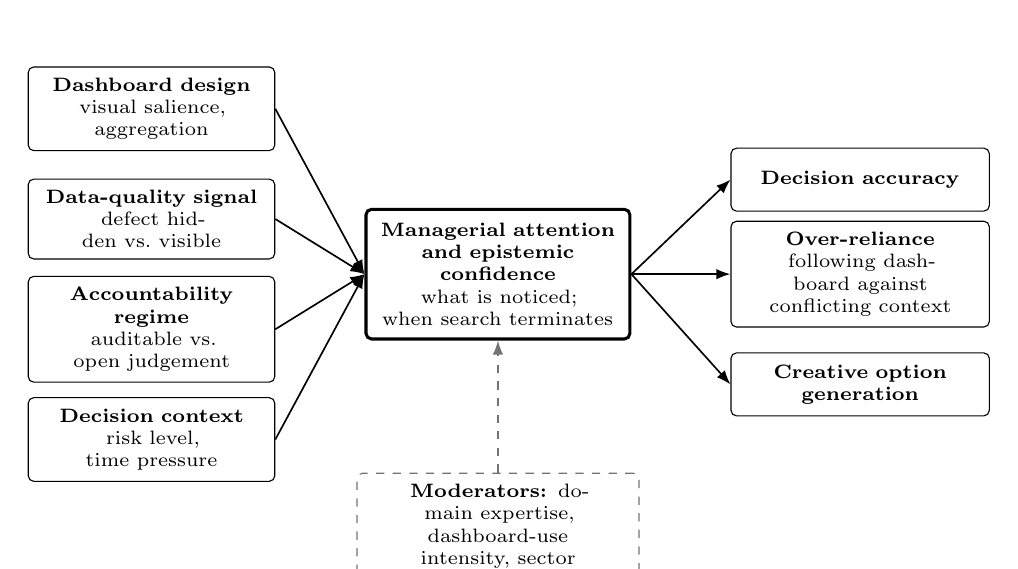
\begin{tikzpicture}[
  every node/.style={font=\scriptsize},
  box/.style={draw=black,rounded corners=2pt,align=center,inner sep=4pt,text width=2.85cm,minimum height=0.95cm},
  med/.style={draw=black,line width=1.1pt,rounded corners=2pt,align=center,inner sep=5pt,text width=3.0cm,minimum height=1.35cm},
  outc/.style={draw=black,rounded corners=2pt,align=center,inner sep=4pt,text width=3.0cm,minimum height=0.8cm},
  mod/.style={draw=black!55,dashed,rounded corners=2pt,align=center,inner sep=4pt,text width=3.3cm},
  ar/.style={-{Latex[length=1.8mm]},line width=0.6pt}]
\node[box] (a1) at (0,2.9) {\textbf{Dashboard design}\\visual salience, aggregation};
\node[box] (a2) at (0,1.5) {\textbf{Data-quality signal}\\defect hidden vs.\ visible};
\node[box] (a3) at (0,0.1) {\textbf{Accountability regime}\\auditable vs.\ open judgement};
\node[box] (a4) at (0,-1.3) {\textbf{Decision context}\\risk level, time pressure};
\node[med] (m) at (4.4,0.8) {\textbf{Managerial attention\\and epistemic confidence}\\\scriptsize what is noticed;\\\scriptsize when search terminates};
\node[outc] (o1) at (9.0,2.0) {\textbf{Decision accuracy}};
\node[outc] (o2) at (9.0,0.8) {\textbf{Over-reliance}\\\scriptsize following dashboard against\\\scriptsize conflicting context};
\node[outc] (o3) at (9.0,-0.6) {\textbf{Creative option\\generation}};
\node[mod] (mo) at (4.4,-2.4) {\textbf{Moderators:} domain expertise,\\dashboard-use intensity, sector};
\foreach \x in {a1,a2,a3,a4} \draw[ar] (\x.east) -- (m.west);
\foreach \y in {o1,o2,o3} \draw[ar] (m.east) -- (\y.west);
\draw[ar,black!55,dashed] (mo.north) -- (m.south);
\end{tikzpicture}
\caption{Initial conceptual framework. Four antecedent conditions act upon managerial attention and
epistemic confidence, which in turn shape three decision outcomes. RQ1 addresses the modelled paths; RQ2
explains why the accountability path operates as it does. Section~5.2 proposes a revision to this model in
the light of the documentary evidence.}
\label{fig:framework}
\end{figure}

\begin{figure}[H]
\centering
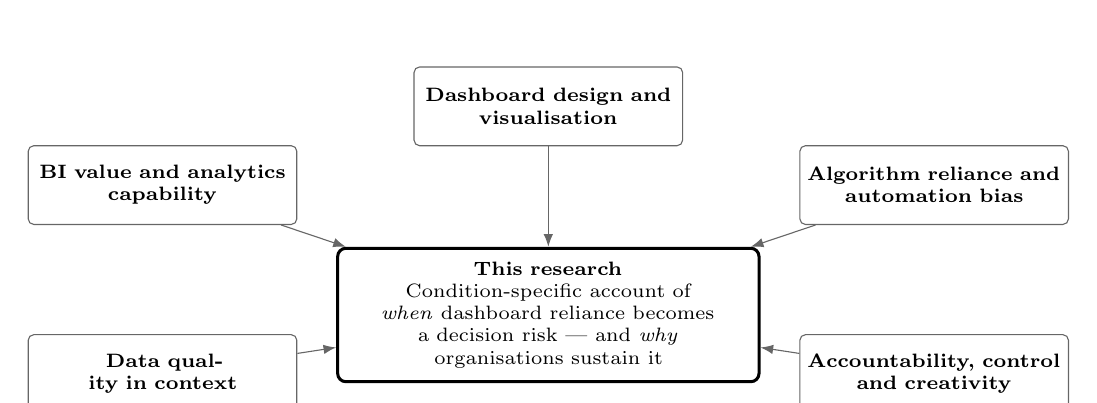
\begin{tikzpicture}[
  every node/.style={font=\scriptsize},
  str/.style={draw=black!60,rounded corners=2pt,align=center,inner sep=3pt,text width=3.2cm,minimum height=1.0cm},
  gapb/.style={draw=black,line width=1.1pt,rounded corners=3pt,align=center,inner sep=5pt,text width=5.0cm,minimum height=1.4cm},
  ar/.style={-{Latex[length=1.6mm]},black!60}]
\node[str] (s1) at (-4.9,2.9) {\textbf{BI value and analytics\\capability}};
\node[str] (s2) at (0,3.9) {\textbf{Dashboard design and\\visualisation}};
\node[str] (s3) at (4.9,2.9) {\textbf{Algorithm reliance and\\automation bias}};
\node[str] (s4) at (-4.9,0.5) {\textbf{Data quality in context}};
\node[str] (s5) at (4.9,0.5) {\textbf{Accountability, control\\and creativity}};
\node[gapb] (g) at (0,1.25) {\textbf{This research}\\Condition-specific account of\\\emph{when} dashboard reliance becomes\\a decision risk --- and \emph{why}\\organisations sustain it};
\foreach \x in {s1,s2,s3,s4,s5} \draw[ar] (\x) -- (g);
\end{tikzpicture}
\caption{Map of contributing research streams and the position of this study. The study sits at the
intersection rather than within any single stream; its distinctiveness lies in the joint treatment of
design, data quality, accountability and creativity as conditions bearing upon one behavioural outcome.}
\label{fig:map}
\end{figure}

\subsection{Hypotheses}

The experimental strand tests the hypotheses in Table~\ref{tab:hyp}. H4 is stated as competing predictions,
since the literature supports both directions; establishing which obtains in dashboard settings is itself a
contribution.

\begin{table}[H]
\centering\small
\caption{Hypotheses, theoretical basis and tested contrast}
\label{tab:hyp}
\begin{tabularx}{\textwidth}{@{}p{0.7cm} X p{3.6cm}@{}}
\toprule
\textbf{ID} & \textbf{Hypothesis} & \textbf{Theoretical basis} \\
\midrule
H1 & Over-reliance is higher when the data-quality defect is hidden than when a freshness or completeness
warning is visible. & Wang and Strong\textsuperscript{\hyperlink{ref74}{74}}; Lyell and Coiera\textsuperscript{\hyperlink{ref41}{41}} \\
H2 & Over-reliance is higher when the decision is framed as auditable than as open managerial judgement,
holding the data constant. & Espeland and Sauder\textsuperscript{\hyperlink{ref24}{24}}; Franco-Santos and Otley\textsuperscript{\hyperlink{ref28}{28}} \\
H3 & Decision accuracy is lower where one key performance indicator dominates visually than under a
balanced multi-indicator view. & Cleveland and McGill\textsuperscript{\hyperlink{ref16}{16}}; Sarikaya \emph{et al.}\textsuperscript{\hyperlink{ref59}{59}} \\
H4a & Higher decision risk \emph{increases} dashboard deference, through a defensibility motive. &
Legitimacy asymmetry, Section~2.5 \\
H4b & Higher decision risk \emph{decreases} dashboard deference, through a verification motive. &
Dietvorst \emph{et al.}\textsuperscript{\hyperlink{ref20}{20}} \\
H5 & Dashboard deference is negatively associated with the number of distinct alternative actions
generated. & Amabile\textsuperscript{\hyperlink{ref2}{2}}; Doshi and Hauser\textsuperscript{\hyperlink{ref21}{21}} \\
H6 & Domain expertise moderates H1, such that more experienced managers challenge hidden-defect dashboards
more frequently. & Kahneman\textsuperscript{\hyperlink{ref34}{34}}; Lebovitz \emph{et al.}\textsuperscript{\hyperlink{ref38}{38}} \\
\bottomrule
\end{tabularx}
\end{table}

%=====================================================================
\section{Research methodology}
%=====================================================================

\subsection{Philosophical position}

The study adopts a critical realist ontology within a pragmatist orientation. Decision errors and their
organisational consequences are treated as real and consequential independently of how they are described,
whilst the mechanisms producing them --- legitimacy, defensibility, professional risk --- are socially
constituted and accessible only through interpretation. This stratified view of reality, in which
observable events are generated by underlying mechanisms that may or may not be
actualised\textsuperscript{\hyperlink{ref8}{8}}, suits a study whose central construct is a mechanism rather than a variable.
Table~\ref{tab:phil} sets out why the principal alternatives were judged less suitable.

\begin{table}[H]
\centering\footnotesize
\caption{Philosophical positions considered, and the basis for the position adopted}
\label{tab:phil}
\begin{tabularx}{\textwidth}{@{}p{2.5cm} X p{4.6cm}@{}}
\toprule
\textbf{Position} & \textbf{Implication for this study} & \textbf{Assessment} \\
\midrule
Positivism & Treats dashboard deference as an observable regularity to be measured and generalised. &
Rejected. It would capture the experimental strand but could not accommodate legitimacy, which is neither
directly observable nor stable across settings. \\
Interpretivism & Treats deference as meaning constructed by professionals in context. & Rejected as a sole
position. It would capture RQ2 but would forbid the controlled comparison that RQ1 requires. \\
Critical realism & Treats observable deference as generated by underlying mechanisms operating under
particular conditions. & \textbf{Adopted.} It licenses both measurement of the event and interpretation of
the mechanism, and it makes conditionality the object of study rather than a nuisance. \\
Pragmatism & Warrants methods by their capacity to answer the question rather than by paradigm allegiance.
& \textbf{Adopted as the practical orientation}, following established mixed-methods
guidance\textsuperscript{\hyperlink{ref19}{19},\hyperlink{ref68}{68}}. \\
\bottomrule
\end{tabularx}
\end{table}

The study reasons abductively: theory specifies initial conditions and hypotheses, and empirical patterns
then refine the framework\textsuperscript{\hyperlink{ref60}{60}}. Section~5.2 is an instance of exactly this, since the
documentary evidence has required the framework to be amended rather than merely confirmed.

\subsection{Design alternatives considered and rejected}

A defensible methodology requires justification not only of what was done but of what was not.
Table~\ref{tab:alt} records the principal alternatives considered.

\begin{table}[H]
\centering\footnotesize
\caption{Design alternatives considered and the basis for rejection}
\label{tab:alt}
\begin{tabularx}{\textwidth}{@{}p{3.3cm} X@{}}
\toprule
\textbf{Alternative} & \textbf{Basis for rejection} \\
\midrule
Field experiment within a single organisation & Would offer the strongest ecological validity, but requires
gatekeeper access to live decision systems, raises acute commercial confidentiality risk, and would confound
the accountability manipulation with a single firm's culture. Not feasible within the dissertation
timetable. \\
Cross-sectional survey of attitudes towards dashboards & Would measure stated beliefs rather than decision
behaviour, and would be exposed to common method bias where predictors and outcome are self-reported from
one instrument\textsuperscript{\hyperlink{ref53}{53}}. The construct of interest is behaviour under conflicting evidence, which a
survey cannot observe. \\
Single in-depth organisational case study & Well suited to mechanism identification\textsuperscript{\hyperlink{ref22}{22},\hyperlink{ref78}{78}}
but incapable of establishing the conditional variation that RQ1 requires, since conditions cannot be
varied within one setting. \\
Interviews alone & Would answer RQ2 but not RQ1, and would rely on retrospective self-report about a
behaviour that participants have little incentive to recall accurately. \\
Secondary analysis of an existing dataset & No public dataset records dashboard-level decision episodes
together with the contextual evidence available at the time. \\
\midrule
\textbf{Adopted: sequential explanatory mixed methods with a concurrent documentary strand} & Experimental
vignettes vary condition whilst holding the decision-maker constant; documentary analysis anchors the
mechanism in real organisational outcomes; interviews explain the observed behaviour. Each strand
compensates for a specific weakness in the others, as Section~3.9 sets out. \\
\bottomrule
\end{tabularx}
\end{table}

\begin{figure}[H]
\centering
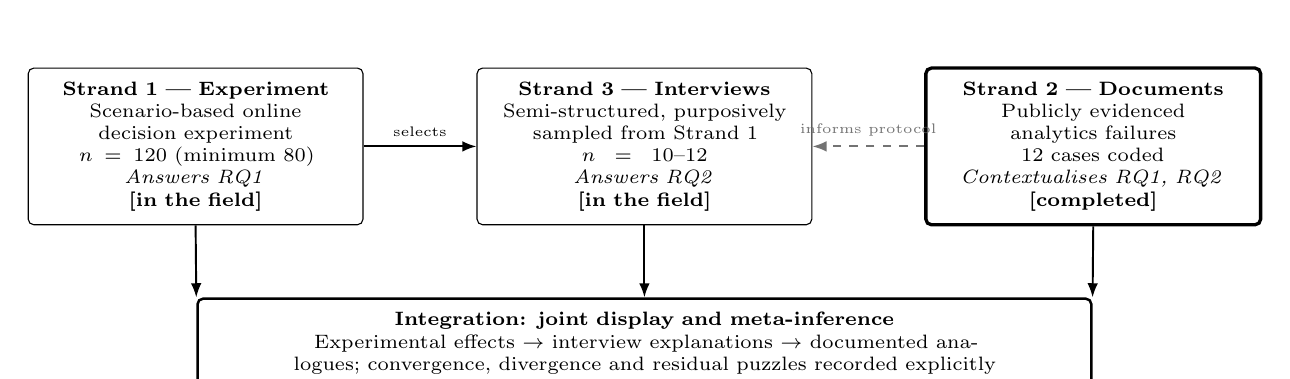
\begin{tikzpicture}[
  every node/.style={font=\scriptsize},
  ph/.style={draw=black,rounded corners=2pt,align=center,inner sep=5pt,text width=3.9cm,minimum height=1.6cm},
  done/.style={draw=black,line width=1.2pt,rounded corners=2pt,align=center,inner sep=5pt,text width=3.9cm,minimum height=1.6cm},
  jd/.style={draw=black,line width=0.9pt,rounded corners=2pt,align=center,inner sep=5pt,text width=11.0cm},
  ar/.style={-{Latex[length=1.8mm]},line width=0.7pt}]
\node[ph] (p1) at (0,0) {\textbf{Strand 1 --- Experiment}\\Scenario-based online\\decision experiment\\$n = 120$ (minimum 80)\\\emph{Answers RQ1}\\\textbf{[in the field]}};
\node[ph] (p3) at (5.7,0) {\textbf{Strand 3 --- Interviews}\\Semi-structured, purposively\\sampled from Strand 1\\$n = 10$--$12$\\\emph{Answers RQ2}\\\textbf{[in the field]}};
\node[done] (p2) at (11.4,0) {\textbf{Strand 2 --- Documents}\\Publicly evidenced\\analytics failures\\12 cases coded\\\emph{Contextualises RQ1, RQ2}\\\textbf{[completed]}};
\node[jd] (j) at (5.7,-2.5) {\textbf{Integration: joint display and meta-inference}\\\scriptsize Experimental effects $\rightarrow$ interview explanations $\rightarrow$ documented analogues; convergence, divergence and residual puzzles recorded explicitly};
\draw[ar] (p1) -- node[above,font=\tiny]{selects} (p3);
\draw[ar,black!55,dashed] (p2) -- node[above,font=\tiny]{informs protocol} (p3);
\draw[ar] (p1.south) -- (j.north west);
\draw[ar] (p3.south) -- (j.north);
\draw[ar] (p2.south) -- (j.north east);
\end{tikzpicture}
\caption{Sequential explanatory design with a concurrent documentary strand. Strand 2 runs first because it
requires neither ethical approval nor recruitment, and its failure patterns sharpen the interview protocol.}
\label{fig:design}
\end{figure}

\subsection{Mapping of research questions to methods}

\begin{table}[H]
\centering\footnotesize
\caption{Mapping of research questions to method, data source, analysis and expected output}
\label{tab:matrix}
\begin{tabularx}{\textwidth}{@{}p{1.0cm} p{2.3cm} X p{2.6cm} p{2.7cm}@{}}
\toprule
\textbf{RQ} & \textbf{Method} & \textbf{Data source} & \textbf{Analysis} & \textbf{Expected output} \\
\midrule
RQ1a & Scenario experiment (Strand 1) & 120 professionals $\times$ 4 vignettes, approximately 480 decision
observations & Mixed-effects logistic regression; odds ratios with 95\% CI & Condition-specific
probabilities of deference \\
RQ1b & Same instrument, count outcome & Number of distinct alternative actions per vignette & Poisson or
negative binomial regression & Estimate of option-set narrowing \\
RQ1 (context) & Documentary analysis (Strand 2) & Regulator notices, inquiry and royal commission reports &
Structured extraction; cross-case matrix & Comparative failure-pattern matrix \textbf{[complete]} \\
RQ2a & Semi-structured interviews (Strand 3) & 10--12 professionals selected on Strand 1 behaviour &
Reflexive thematic analysis & Mechanism themes for deference and challenge \\
RQ2b & Interviews and documents & Interview accounts triangulated against control failures & Pattern
matching across strands & Conditions enabling challenge; governance framework \\
\bottomrule
\end{tabularx}
\end{table}

\subsection{Strand 1: scenario-based decision experiment}

\subsubsection{Instrument design}

The instrument follows established experimental vignette methodology, which is well suited to examining
judgement and decision-making where the factors of interest cannot ethically or practically be manipulated
in the field\textsuperscript{\hyperlink{ref1}{1},\hyperlink{ref5}{5}}. The design is a $2\times2\times2$ within-subjects vignette
experiment. Each vignette presents a realistic dashboard image together with a short decision brief
containing a contextual cue that conflicts with the dashboard's headline signal; for instance, a supply
chain dashboard showing demand as stable whilst a named regional depot reports repeated delivery failures.
Factors and measures are set out in Table~\ref{tab:factors}.

Two design decisions follow directly from the appraisal in Section~2.7. Participants are practising
professionals rather than students, addressing the ecological validity concern; and accountability framing
is manipulated explicitly rather than held constant, addressing the omission that makes generic
advice-taking studies difficult to transfer.

\begin{table}[H]
\centering\footnotesize
\caption{Experimental factors, levels and operationalisation}
\label{tab:factors}
\begin{tabularx}{\textwidth}{@{}p{3.0cm} p{3.1cm} X@{}}
\toprule
\textbf{Factor} & \textbf{Levels} & \textbf{Operationalisation} \\
\midrule
Decision risk & High / Low & Stated financial and reputational consequence of an incorrect decision \\
Data-quality signal & Hidden / Visible & Presence or absence of a banner disclosing that the feed is six
days stale and twelve per cent incomplete \\
Accountability framing & Auditable / Open judgement & Instruction that the decision will be recorded and
reviewed against the dashboard, as against recorded as a managerial judgement \\
Metric salience \emph{(between subjects)} & Single dominant KPI / Balanced multi-indicator & Visual emphasis
manipulated through size and position \\
\midrule
\multicolumn{3}{@{}l}{\textbf{Measured outcomes}}\\
Over-reliance \emph{(primary)} & Binary & Chose the dashboard-consistent action despite the conflicting
contextual cue \\
Decision accuracy & Binary & Chose the action correct on all available evidence \\
Creative option generation & Count & Number of distinct alternative actions listed, double-coded \\
Confidence & Seven-point scale & Self-rated confidence in the chosen action \\
Verification intent & Binary & Whether additional data were requested before deciding \\
\midrule
\multicolumn{3}{@{}l}{\textbf{Covariates:} sector, years of experience, seniority, dashboard-use frequency,
self-rated analytics familiarity}\\
\bottomrule
\end{tabularx}
\end{table}

\subsubsection{Sampling and sample size}

Participants are working professionals using dashboards, KPI reports or BI tools in a managerial or
analytical capacity in finance, consulting, operations, logistics, technology or analytics roles.
Recruitment is non-probability purposive with snowball extension. A screening question enforces the
inclusion criterion of dashboard use at least weekly during the preceding twelve months.

\nbox{Sample size justification}{%
\textbf{Target $N = 120$ completed responses; minimum viable $N = 80$.} Each participant completes four of
eight vignettes, randomised and counterbalanced, yielding approximately 480 decision observations at target.
For a two-proportion comparison of over-reliance rates of 0.35 against 0.60 at $\alpha = .05$ (two-tailed)
and power of $.80$, approximately 123 independent observations are required.\textsuperscript{\hyperlink{ref18}{18},\hyperlink{ref25}{25}} Since the design is
within-subjects, the effective requirement is inflated by the design effect $1+(m-1)\rho$; at $m=4$ and an
intra-class correlation of $\rho = .20$ the design effect is 1.60, implying roughly 50 participants for that
single contrast. The target of 120 therefore provides margin to detect differences of approximately 20
percentage points, to estimate the three-way condition structure rather than a single contrast, and to test
the expertise moderation in H6.}

\subsubsection{Piloting and analysis}

The instrument is piloted with eight to ten respondents from the target population plus two academic
reviewers, checking that the contextual cue is noticed without dominating, that the data-quality banner is
legible without becoming a demand characteristic, that completion time remains under twelve minutes, and
that double coding of the creativity count is reliable. Attention checks, a minimum-time filter and
manipulation checks guard against inattentive responding and failed manipulation.

The primary model is a mixed-effects logistic regression with a random intercept for participant,
predicting over-reliance from decision risk, data-quality signal, accountability framing, metric salience
and pre-specified interactions. Alternative-option counts are modelled by Poisson or negative binomial
regression with overdispersion tested. Where the mixed model's assumptions cannot be satisfied, the
pre-committed fallback is logistic regression with cluster-robust standard errors, supplemented by McNemar
tests for within-subject paired contrasts. Effect sizes are reported alongside significance values, and the
analysis plan was fixed before data collection to prevent selective reporting.

\subsection{Strand 2: documentary analysis}

\subsubsection{Rationale and admissibility}

Documentary analysis is appropriate where the phenomenon of interest leaves a durable, independently
verifiable trace and where the researcher cannot be present at the events
concerned\textsuperscript{\hyperlink{ref9}{9},\hyperlink{ref36}{36}}. Both conditions hold here: organisational analytics failures of
consequence generate statutory investigation, and no researcher could observe such an episode as it
unfolds.

Only documents whose independent existence may be verified are admissible: regulator enforcement notices
and consent orders; statutory public inquiry and royal commission reports; independent reviews commissioned
by regulators; national audit office and parliamentary committee reports; and listed-company annual reports
and restatement disclosures. Press coverage may be used to locate a case but never as the sole evidential
basis for a coded judgement. Cases were selected by maximum-variation sampling across sector and failure
type to avoid an all-finance sample, requiring that the event occurred between 2010 and 2026, that primary
documentation is available in English, and that the facts are settled rather than contested in ongoing
proceedings.

\subsubsection{Evidential grading and coding reliability}

A refinement adopted during coding, and one not commonly reported at this level, is the explicit grading of
evidential strength. Grade A denotes a case documented by a dedicated statutory investigation, royal
commission or regulatory enforcement notice. Grade B denotes a case documented by official organisational
disclosure together with parliamentary or regulatory scrutiny but without a dedicated independent
investigation. Of the twelve cases, ten are Grade A and two are Grade B. Grading is reported transparently
so that a reader may discount the weaker cases.

Each case was coded against the fixed frame in Table~\ref{tab:frame}, with a verbatim supporting quotation
and page reference recorded for every judgement. A second coder independently coded a thirty per cent
subsample; agreement will be reported as Cohen's $\kappa$\textsuperscript{\hyperlink{ref17}{17}} and interpreted against conventional
benchmarks\textsuperscript{\hyperlink{ref37}{37}}, with disagreements resolved by discussion and the resolution logged.

\begin{table}[H]
\centering\small
\caption{Structured extraction frame for the documentary analysis}
\label{tab:frame}
\begin{tabularx}{\textwidth}{@{}p{3.4cm} X@{}}
\toprule
\textbf{Dimension} & \textbf{Coded content} \\
\midrule
Failure type & Accuracy / timeliness / completeness / consistency / model logic \\
Signal visibility & Was the defect detectable from the interface or report at the point of use? Coded
silent, partial or visible \\
Detection lag & Elapsed time between failure onset and organisational recognition \\
Human challenge & Was the output challenged? By whom? Was the challenge escalated, ignored or overridden? \\
Legitimacy asymmetry & Evidence that system output was treated as more authoritative than human accounts;
coded strong, moderate or weak \\
Control mechanism & Warnings, overrides, reconciliation or governance that existed, and why they failed \\
Organisational impact & Financial, operational, regulatory and human consequences \\
Evidential grade & A or B, as defined above \\
\bottomrule
\end{tabularx}
\end{table}

\subsection{Strand 3: semi-structured interviews}

Ten to twelve interviews will be conducted, with a floor of eight, reflecting evidence that thematic
saturation in relatively homogeneous samples typically emerges within approximately twelve
interviews\textsuperscript{\hyperlink{ref30}{30}} whilst remaining feasible within the timetable\textsuperscript{\hyperlink{ref11}{11}}.

Participants are selected purposively from Strand 1 respondents consenting to follow-up, and sampled upon
\emph{observed behaviour} rather than convenience: strong deference across conditions; consistent challenge
behaviour; and inconsistent response to data-quality warnings. This behaviour-linked sampling is the
mechanism making the design genuinely explanatory rather than merely sequential, since it permits the
interview to interrogate a specific decision the participant actually made rather than a decision they
report having made. Interviews last thirty to forty minutes and are conducted online. Analysis follows
reflexive thematic analysis\textsuperscript{\hyperlink{ref10}{10}}, with NVivo supporting coding, memoing and theme development.

\subsection{Quality criteria}

Table~\ref{tab:quality} maps the quality criteria applicable to each strand onto the specific actions taken,
following the convention of treating quantitative and qualitative criteria
separately\textsuperscript{\hyperlink{ref39}{39},\hyperlink{ref60}{60}}.

\begin{table}[H]
\centering\footnotesize
\caption{Quality criteria and corresponding design actions}
\label{tab:quality}
\begin{tabularx}{\textwidth}{@{}p{2.1cm} p{3.0cm} X@{}}
\toprule
\textbf{Strand} & \textbf{Criterion} & \textbf{Action taken} \\
\midrule
1 & Internal validity & Randomised and counterbalanced vignette allocation; within-subjects design holding
the decision-maker constant; manipulation checks \\
1 & Construct validity & Two independent coders for the creativity count; attention and comprehension
checks; pilot testing of cue salience \\
1 & External validity & Practising professionals rather than students; realistic dashboards; acknowledged
limitation that vignette stakes remain lower than real ones \\
1 & Common method bias & Outcome is a behavioural choice rather than a self-report; predictors are
experimentally manipulated rather than measured\textsuperscript{\hyperlink{ref53}{53}} \\
2 & Documentary authenticity & Only independently verifiable primary documents admitted; evidential grading
applied and reported \\
2 & Coding reliability & Fixed extraction frame; thirty per cent double coding; Cohen's $\kappa$ reported \\
3 & Credibility & Behaviour-linked sampling; member checking of summarised themes \\
3 & Dependability & Audit trail of coding decisions and analytic memos \\
3 & Transferability & Thick description of participant sector, role and context \\
3 & Reflexivity & The researcher's analytics training creates a plausible bias towards reading deference as
error; coding therefore actively seeks accounts in which deference proved correct \\
\bottomrule
\end{tabularx}
\end{table}

\subsection{Ethical considerations}

Ethical approval, the fieldwork risk assessment and the GDPR assessment were completed and approved before
any primary data collection commenced, in accordance with the University's Code of Good Practice in
Research. The study is additionally conducted in accordance with the MRS Code of Conduct\textsuperscript{\hyperlink{ref43}{43}}, whose
provisions on informed consent, non-deception and the avoidance of harm apply directly to research with
professional participants. Four design-specific matters warrant particular mention.

\emph{Participants must not be made to feel personally evaluated.} The experiment presents decision problems
having better and worse answers, and participants are professionals whose competence forms part of their
identity. The study is therefore framed throughout as research into how dashboards are designed and used
and never into individual managerial ability. No participant receives a score; no individual-level feedback
is given; results are reported only in aggregate; and the debrief explains that the scenarios were
deliberately constructed so that the dashboard could mislead, so that following it was reasonable rather
than incompetent. A degree of concealment of the manipulation is unavoidable if the behaviour is to be
observed at all, and this is handled by full disclosure at debrief rather than by active deception at any
point.

\emph{Commercial confidentiality and professional risk.} Interviewees work in regulated, client-facing or
commercially sensitive environments. The information sheet and verbal preamble state explicitly that
participants must not disclose confidential organisational information, proprietary dashboard designs,
client data, named clients or commercially sensitive decision processes. Should a participant begin to
disclose such material, the interviewer will interrupt and the passage will be excluded from transcription.
Employers are described by sector and size band only.

\emph{Data protection.} Data are held on University-provided encrypted storage; transcripts are
pseudonymised at the point of transcription; recordings are deleted following verification; and processing
is on the basis of consent under the UK GDPR. Participants may withdraw without giving a reason and may
request deletion of their data up to two weeks after participation, after which anonymisation renders
retrieval impossible.

\emph{Secondary data and the dignity of those harmed.} Strand 2 uses only material already in the public
domain. Because several cases involve identifiable individuals who suffered serious harm --- the Post Office
and Robodebt cases most obviously --- the analysis focuses upon organisational and system-level control
failures rather than upon individual conduct, and treats human consequences with proportionate care rather
than as illustrative colour.

\subsection{Methodological limitations}

Four limitations are stated explicitly, in keeping with the expectation that limitations be made explicit
rather than implied.

Firstly, the vignette design measures stated decisions in a low-stakes setting. However realistic the
dashboard, no participant loses money or standing by choosing wrongly, and the accountability manipulation
is therefore a simulation of accountability rather than the thing itself. The direction of the resulting
bias is towards understating deference, since the defensibility motive is weaker in the laboratory than in
the organisation.

Secondly, non-probability recruitment limits generalisation, and self-selection may over-represent
professionals already reflective about analytics. Sector and seniority distributions will be reported
transparently rather than claimed as representative.

Thirdly, the documentary strand is subject to severe survivorship bias, discussed at length in
Section~5.3. It establishes the anatomy of failure, not its base rate.

Fourthly, the three strands are not equally weighted in evidential strength. The documentary strand rests
upon authoritative primary documents but a small purposive sample; the experimental strand upon a larger
sample but an artificial task; the interview strand upon rich accounts but retrospective self-report.
Integration must therefore be interpretive rather than arithmetic, and no strand is treated as validating
another in a strong sense.

%=====================================================================
\section{Findings}
%=====================================================================

\subsection{Overview}

The documentary strand has been completed in full and is reported in Section~4.2. The experimental and
interview strands remain in the field, and sections depending upon them are marked accordingly.
Section~4.5 sets out the joint display through which the three strands will be integrated.

\subsection{Strand 2: documentary analysis of twelve organisational failures}

\subsubsection{The case sample}

Twelve cases satisfied the inclusion criteria and were coded in full, spanning nine sectors and four
jurisdictions (Table~\ref{tab:cases}). Every case is anchored to a document whose independent existence may
be verified, in accordance with the admissibility rule of Section~3.6.

\begin{table}[H]
\centering\footnotesize
\caption{The documentary case sample, with evidential grade and primary source}
\label{tab:cases}
\begin{tabularx}{\textwidth}{@{}p{0.7cm} p{3.0cm} p{2.6cm} p{1.5cm} p{0.7cm} X@{}}
\toprule
\textbf{ID} & \textbf{Case} & \textbf{Sector} & \textbf{Period} & \textbf{Gr.} & \textbf{Primary source} \\
\midrule
C1 & Post Office Horizon & Postal / retail (UK) & 1999–2019 & A & Post Office Horizon IT Inquiry (2025) Final Report, Vol. 1 \\
C2 & NATS flight planning & Aviation (UK) & 2023 & A & Civil Aviation Authority (2024) CAP2993 \\
C3 & Citibank risk data & Banking (US) & 2013–2020 & A & OCC (2020) News Release NR 2020-132 \\
C4 & PHE case undercount & Public health (UK) & 2020 & B & Official statements and parliamentary scrutiny (2020) \\
C5 & Robodebt & Welfare (AU) & 2015–2020 & A & Royal Commission into the Robodebt Scheme (2023) Report \\
C6 & TSB migration & Banking (UK) & 2018 & A & FCA (2022) Final Notice: TSB Bank plc \\
C7 & Knight Capital & Trading (US) & 2012 & A & SEC (2013) Order 34-70694 \\
C8 & Ofqual grading & Education (UK) & 2020 & A & Office for Statistics Regulation (2021) Review \\
C9 & Dutch childcare benefits & Welfare / tax (NL) & 2013–2020 & A & Autoriteit Persoonsgegevens (2021) Enforcement decision \\
C10 & Goldman Sachs reporting & Banking (UK) & 2007–2017 & A & FCA (2019) Final Notice: Goldman Sachs International \\
C11 & Zillow Offers & Real estate / tech (US) & 2021 & B & Zillow Group (2021) Q3 shareholder letter (SEC filing) \\
C12 & Boeing 737 MAX (MCAS) & Aerospace (US) & 2012–2019 & A & US House Committee on Transportation and Infrastructure (2020) Final Report \\
\bottomrule
\end{tabularx}
\end{table}

\subsubsection{Failure types and visibility of the defect}

Figure~\ref{fig:failtype} presents the distribution of failure types, disaggregated by whether the defect
was detectable at the point of use. Two observations follow.

Firstly, model-logic failures dominate, accounting for eight of twelve cases. The problem was most commonly
not that a number had been entered wrongly, but that the system was doing exactly what it had been designed
to do upon a rule that was itself inappropriate for the situation. Robodebt provides the clearest
illustration: averaging annual income across fortnightly periods was arithmetically faultless and
substantively wrong for anybody whose earnings varied across the year\textsuperscript{\hyperlink{ref56}{56}}. The Ofqual
standardisation model of 2020 likewise executed its specification correctly whilst producing outcomes that
could not be defended at the level of the individual pupil\textsuperscript{\hyperlink{ref47}{47}}.

Secondly, and more importantly for the argument advanced here, the defect was silent at the point of use in
seven cases and only partially visible in a further four. In one case only --- the TSB migration of 2018,
where customers were immediately unable to access their accounts --- was the failure plainly visible to
those affected\textsuperscript{\hyperlink{ref27}{27}}. This provides direct documentary support for the premise of Section~2.4, namely
that data and model defects do not announce themselves.

\begin{figure}[H]
\centering

\includegraphics[width=0.82\textwidth]{fig/f_failtype.pdf}
\caption{Distribution of failure types across the twelve cases, disaggregated by whether the defect was
detectable at the point of use. Model-logic failures dominate, and the majority of defects were silent to
the person relying upon the output.}
\label{fig:failtype}
\end{figure}

\subsubsection{Detection lag and the cost of silence}

If a defect gives no perceptual cue, one would expect it to persist. Figure~\ref{fig:lag} plots detection
lag on a logarithmic scale, shaded by signal visibility, and Figure~\ref{fig:box} summarises the same
relationship.

The pattern is stark. Cases in which the defect was silent persisted for a median of several years: Post
Office Horizon for approximately sixteen years\textsuperscript{\hyperlink{ref54}{54}}; Goldman Sachs International's transaction
reporting failures for some nine and a half years, covering approximately 213.6 million reportable
transactions\textsuperscript{\hyperlink{ref26}{26}}; the Dutch childcare benefits risk classification for around seven
years\textsuperscript{\hyperlink{ref6}{6}}; and the Boeing 737 MAX manoeuvring characteristics augmentation system for roughly six
years from specification to the second accident\textsuperscript{\hyperlink{ref71}{71}}. By contrast, cases producing a perceptible
signal were recognised within hours or days: Knight Capital within approximately forty-five
minutes\textsuperscript{\hyperlink{ref61}{61}}, the NATS flight-planning failure within a few hours\textsuperscript{\hyperlink{ref15}{15}}, and the Public Health
England case undercount within roughly eight days.

Care is required about what this comparison shows. The two groups differ in more than signal visibility:
silent defects tend to arise in slower-moving administrative processes, whereas signalled defects tend to
arise in real-time operational systems, so exposure time is confounded with visibility. The comparison is
therefore suggestive rather than causal, and no significance test is offered upon twelve purposively
selected cases, since the sampling strategy was designed for variation rather than for representativeness.
What may fairly be said is that the documentary record is entirely consistent with the proposition that
visibility governs the speed of correction, and that the proposition is worth testing experimentally ---
which is what H1 does.

\begin{figure}[H]
\centering

\includegraphics[width=0.86\textwidth]{fig/f_lag.pdf}
\caption{Detection lag by case, ordered from shortest to longest and shaded by visibility of the defect at
the point of use. The horizontal axis is logarithmic. Silent defects cluster at the long-duration end.}
\label{fig:lag}
\end{figure}

\begin{figure}[H]
\centering

\includegraphics[width=0.58\textwidth]{fig/f_box.pdf}
\caption{Detection lag for silent as against partially or fully signalled defects, with individual cases
overlaid. The difference of several orders of magnitude is descriptive of this purposive sample and is not
an estimate of any population parameter.}
\label{fig:box}
\end{figure}

\subsubsection{The principal finding: challenge was raised and overridden}

The most consequential finding of this strand concerns not detection but authority.

In nine of the twelve cases a human being challenged the system output, and the challenge was subsequently
overridden, ignored or not acted upon. In one case only --- Zillow's decision to wind down its iBuying
operation once forecasting losses became apparent --- was a challenge raised and acted upon in a manner that
limited the harm\textsuperscript{\hyperlink{ref79}{79}}. In two cases no challenge was raised at all, and in both the defect was
entirely silent, so that there was nothing for anybody to challenge.

Figure~\ref{fig:challenge} presents this distribution cross-tabulated with the coded strength of legitimacy
asymmetry. Every case coded as exhibiting a strong asymmetry falls within the ``raised and overridden''
group.

The qualitative texture of these overrides is instructive. Sub-postmasters challenged Horizon's figures
consistently over many years, and the response was prosecution rather than investigation\textsuperscript{\hyperlink{ref54}{54}}. In the
Robodebt scheme, internal legal advice questioning the lawfulness of income averaging was obtained and then
set aside\textsuperscript{\hyperlink{ref56}{56}}. Engineering concerns regarding the 737 MAX system's reliance upon a single
angle-of-attack sensor were raised internally without altering the certification outcome\textsuperscript{\hyperlink{ref71}{71}}.
Knight Capital is instructive in a different way: the firm's systems generated ninety-seven automated email
messages within the relevant window, but these were not designed as system alerts and were not treated as
such\textsuperscript{\hyperlink{ref61}{61}}. The information was present; the authority to act upon it was not.

This is precisely the pattern that legitimacy asymmetry predicts. The binding constraint upon correction
was not the availability of contrary information but the relative institutional standing of the system
output as against the human objection.

\begin{figure}[H]
\centering

\includegraphics[width=0.88\textwidth]{fig/f_challenge.pdf}
\caption{Outcome of human challenge across the twelve cases, cross-tabulated with the coded strength of
legitimacy asymmetry. In nine of twelve cases a challenge was raised and did not prevent the harm.}
\label{fig:challenge}
\end{figure}

\subsubsection{Cross-case matrix}

Table~\ref{tab:coded} presents the full coded matrix and Figure~\ref{fig:heat} renders the same information
visually. Reading the heat map column by column, the cases producing the gravest human consequences ---
Horizon, Robodebt, the Dutch childcare benefits scheme and the 737 MAX --- share a common signature: a
silent defect, a strong legitimacy asymmetry, suppressed challenge and a control mechanism either absent or
bypassed. This four-way co-occurrence is the empirical shape of the mechanism that Section~2.5 describes
theoretically.

\begin{table}[H]
\centering\footnotesize
\caption{Cross-case coded matrix for the documentary strand}
\label{tab:coded}
\begin{tabularx}{\textwidth}{@{}p{0.7cm} p{1.9cm} p{1.4cm} p{1.2cm} X p{1.5cm} p{2.4cm}@{}}
\toprule
\textbf{ID} & \textbf{Failure type} & \textbf{Signal} & \textbf{Lag} & \textbf{Human challenge} &
\textbf{Asym.} & \textbf{Control} \\
\midrule
C1 & Model logic & Silent & 16 yr & Raised, overridden & Strong & Present, ineffective \\
C2 & Model logic & Partial & $\sim$4 hr & Raised, slow escalation & Moderate & Present, ineffective \\
C3 & Consistency & Silent & 7 yr & Raised, overridden & Moderate & Present, ineffective \\
C4 & Completeness & Silent & 8 d & Not raised & Moderate & Absent \\
C5 & Model logic & Silent & 5 yr & Raised, overridden & Strong & Present, bypassed \\
C6 & Consistency & Visible & 1 d & Raised, overridden & Weak & Present, ineffective \\
C7 & Model logic & Partial & <2 hr & Alerts issued, ignored & Weak & Absent \\
C8 & Model logic & Partial & 4 d & Raised, overridden & Strong & Present, ineffective \\
C9 & Model logic & Silent & 7 yr & Raised, overridden & Strong & Absent \\
C10 & Accuracy & Silent & 9 yr & Not raised & Weak & Present, ineffective \\
C11 & Model logic & Partial & 6 mo & Raised, acted upon & Moderate & Present, effective \\
C12 & Model logic & Silent & 6 yr & Raised, overridden & Strong & Present, bypassed \\
\bottomrule
\end{tabularx}
\end{table}

\begin{figure}[H]
\centering

\includegraphics[width=\textwidth]{fig/f_heat.pdf}
\caption{Cross-case heat map of the four principal coded dimensions, where H denotes high, M moderate and L
low. The four cases producing the most severe human consequences share the same signature across all four
dimensions.}
\label{fig:heat}
\end{figure}

\subsubsection{Control mechanisms and why they failed}

In one case only was a control mechanism both present and effective. In six cases a control existed but
proved ineffective, in two it existed and was bypassed, and in three it was absent. The Public Health
England undercount is illuminating because the missing control was so elementary: no reconciliation was
performed between the number of records dispatched and the number received, so a silent truncation at the
row limit of an obsolete file format passed unnoticed for roughly a week.

The wider lesson, which the governance framework of Section~6.2 must accommodate, is that the controls that
failed were overwhelmingly \emph{detective} rather than \emph{authorising}. Organisations possessed
mechanisms for spotting problems. What they generally lacked was a mechanism conferring standing upon the
person who had spotted one.

\subsection{Strand 1: experimental findings}

\pend{awaiting Strand 1 data}{%
This section will report the scenario-based decision experiment. The structure has been fixed in advance of
data collection, and the analysis script has been written and tested upon simulated data so that only
execution remains.\\[4pt]
\textbf{4.3.1 Sample and data screening} --- response and completion rates, exclusions for failed attention
checks and sub-threshold completion times, final analytic $N$, and participant profile by sector, seniority
and dashboard-use frequency.\\[3pt]
\textbf{4.3.2 Descriptive results} --- over-reliance and accuracy rates by experimental condition, with a
grouped bar chart across the eight vignette cells and a histogram of alternative-option counts.\\[3pt]
\textbf{4.3.3 Hypothesis tests} --- mixed-effects logistic regression of over-reliance upon decision risk,
data-quality signal, accountability framing and metric salience, reported as odds ratios with 95 per cent
confidence intervals and a forest plot. H4a and H4b will be adjudicated here.\\[3pt]
\textbf{4.3.4 Option generation} --- count model of alternatives generated, testing H5.\\[3pt]
\textbf{4.3.5 Moderation by expertise} --- test of H6 as an interaction term with a marginal effects plot.}

\subsection{Strand 3: interview findings}

\pend{awaiting Strand 3 data}{%
This section will report the thematic analysis of the semi-structured interviews.\\[4pt]
\textbf{4.4.1 Participant profile} --- sector, role, seniority and the Strand 1 behavioural profile upon
which each participant was selected, in pseudonymised form.\\[3pt]
\textbf{4.4.2 Themes} --- four to six named themes with illustrative quotations and a thematic map. The
anticipated themes, held loosely and open to disconfirmation, are: defensibility; verification cost;
suppressed intuition; permission to challenge; and the measured option.\\[3pt]
\textbf{4.4.3 Disconfirming accounts} --- instances in which deference proved correct and challenge would
have been mistaken, reported explicitly rather than set aside.}

\subsection{Integration across the three strands}

\pend{awaiting Strands 1 and 3}{%
The three strands will be integrated through the joint display of Table~\ref{tab:joint}, whose first column
is already populated from the completed documentary strand. Divergences between strands will be recorded
rather than smoothed away.}

\begin{table}[H]
\centering\footnotesize
\caption{Joint display, with the documentary column populated}
\label{tab:joint}
\begin{tabularx}{\textwidth}{@{}p{3.4cm} p{3.2cm} p{3.2cm} X@{}}
\toprule
\textbf{Documented pattern (Strand 2, complete)} & \textbf{Experimental finding (Strand 1, pending)} &
\textbf{Explanation (Strand 3, pending)} & \textbf{Provisional meta-inference} \\
\midrule
Silent defects persisted for years; signalled defects were caught within days & \emph{H1: over-reliance
higher when the defect is hidden} & \emph{Why practitioners treat absence of warning as assurance} & Absence
of a warning appears to be read as positive assurance rather than as absence of information \\
\addlinespace
Challenge was raised and overridden in nine of twelve cases & \emph{H2: auditable framing raises deference}
& \emph{Whether defensibility is the stated reason} & Legitimacy asymmetry may operate at both individual
and institutional levels \\
\addlinespace
Controls were detective rather than authorising & \emph{Verification intent by condition} & \emph{Conditions
under which challenge is permitted} & Governance may need to confer standing, not merely detection
capability \\
\bottomrule
\end{tabularx}
\end{table}

%=====================================================================
\section{Discussion}
%=====================================================================

\nbox{Status of this chapter}{%
The discussion interprets the completed documentary strand against the conceptual framework and identifies
the points at which the experimental and interview findings will corroborate or complicate the present
reading. It will be rewritten once all three strands are available.}

\subsection{What the documentary evidence supports}

Three propositions from Section~2 receive preliminary support.

\emph{Defects are behaviourally silent.} Eleven of twelve cases were coded silent or only partially visible,
and the association between silence and long persistence is pronounced. This lends weight to theorising data
quality as a problem of perception rather than only of measurement --- a reframing that the dimensional
tradition\textsuperscript{\hyperlink{ref67}{67},\hyperlink{ref74}{74}} does not itself supply.

\emph{The constraint is authority rather than detection.} This is the finding that most substantially
advances the framework, and it is discussed in Section~5.2.

\emph{Legitimacy asymmetry is observable outside the laboratory.} The construct was developed on
essentially theoretical grounds from reactivity and performance-management
research\textsuperscript{\hyperlink{ref24}{24},\hyperlink{ref28}{28}}. Its empirical signature --- system output treated as more
authoritative than human accounts --- is visible in all five cases coded as exhibiting a strong asymmetry,
and most starkly in Horizon, where system data was accorded sufficient authority to sustain criminal
prosecutions against the contrary testimony of those concerned\textsuperscript{\hyperlink{ref54}{54}}.

\subsection{Revising the conceptual framework}

Prior to this analysis, the working assumption embedded in Figure~\ref{fig:framework} was that reduced
attentional sampling --- the mechanism Parasuraman and Manzey describe\textsuperscript{\hyperlink{ref49}{49}} --- is the
principal route by which dashboards displace judgement. The documentary record indicates that this is at
best a partial account. In nine of twelve cases attention was not the problem. Somebody noticed. What failed
was the conversion of a noticing into an organisational decision.

The framework therefore requires an explicit distinction between two failure modes, which
Figure~\ref{fig:revised} incorporates.

\emph{Detection failure} occurs where the defect is silent and no cue triggers effortful processing. Its
antecedents are dashboard design and data-quality signal visibility; its remedy is disclosure, provenance
and uncertainty display. This is the failure mode that the existing literature describes well.

\emph{Authority failure} occurs where the defect is noticed and articulated but the objection lacks
institutional standing sufficient to alter the decision. Its antecedent is the accountability regime; its
remedy is not better information but a governance route by which a contextual objection becomes an
auditable input. This failure mode is largely absent from the dashboard and automation-bias literatures,
which is unsurprising given their origins in single-operator settings where the operator both notices and
decides.

The theoretical value of the distinction is that the two modes respond to different interventions and can
be present independently. A dashboard may be scrupulously transparent about data quality and still sit
within an organisation where disagreement carries career risk; conversely, an organisation may have
excellent escalation culture and still be blind to a silent truncation. Cognitive forcing
functions\textsuperscript{\hyperlink{ref12}{12}} address detection; they do nothing for authority. This, arguably, is why
interventions of that kind have shown promise in laboratory settings whilst organisational analytics
failures have continued.

\begin{figure}[H]
\centering
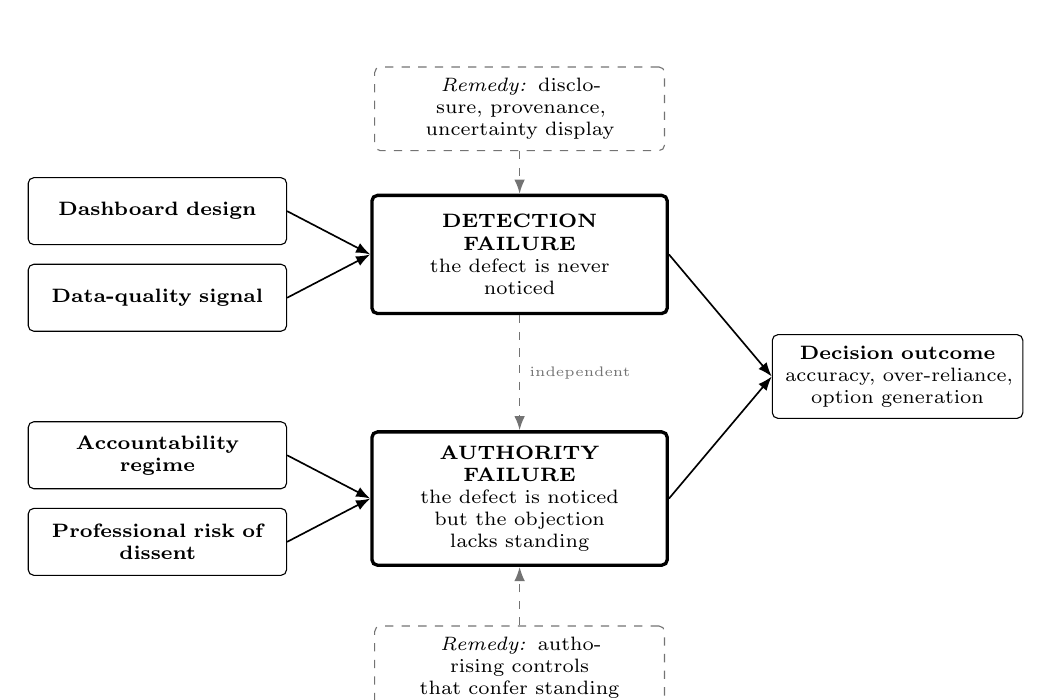
\begin{tikzpicture}[
  every node/.style={font=\scriptsize},
  ant/.style={draw=black,rounded corners=2pt,align=center,inner sep=4pt,text width=3.0cm,minimum height=0.85cm},
  mode/.style={draw=black,line width=1.2pt,rounded corners=2pt,align=center,inner sep=5pt,text width=3.4cm,minimum height=1.5cm},
  outc/.style={draw=black,rounded corners=2pt,align=center,inner sep=4pt,text width=2.9cm,minimum height=0.8cm},
  rem/.style={draw=black!55,dashed,rounded corners=2pt,align=center,inner sep=4pt,text width=3.4cm},
  ar/.style={-{Latex[length=1.8mm]},line width=0.6pt}]
\node[ant] (d1) at (0,2.4) {\textbf{Dashboard design}};
\node[ant] (d2) at (0,1.3) {\textbf{Data-quality signal}};
\node[ant] (a1) at (0,-0.7) {\textbf{Accountability regime}};
\node[ant] (a2) at (0,-1.8) {\textbf{Professional risk of\\dissent}};
\node[mode] (m1) at (4.6,1.85) {\textbf{DETECTION FAILURE}\\\scriptsize the defect is never\\\scriptsize noticed};
\node[mode] (m2) at (4.6,-1.25) {\textbf{AUTHORITY FAILURE}\\\scriptsize the defect is noticed\\\scriptsize but the objection\\\scriptsize lacks standing};
\node[outc] (o) at (9.4,0.3) {\textbf{Decision outcome}\\\scriptsize accuracy, over-reliance,\\\scriptsize option generation};
\node[rem] (r1) at (4.6,3.7) {\emph{Remedy:} disclosure, provenance,\\uncertainty display};
\node[rem] (r2) at (4.6,-3.4) {\emph{Remedy:} authorising controls\\that confer standing};
\draw[ar] (d1.east) -- (m1.west); \draw[ar] (d2.east) -- (m1.west);
\draw[ar] (a1.east) -- (m2.west); \draw[ar] (a2.east) -- (m2.west);
\draw[ar] (m1.east) -- (o.west); \draw[ar] (m2.east) -- (o.west);
\draw[ar,black!55,dashed] (r1.south) -- (m1.north);
\draw[ar,black!55,dashed] (r2.north) -- (m2.south);
\draw[ar,black!55,dashed] (m1.south) -- node[right,font=\tiny]{independent} (m2.north);
\end{tikzpicture}
\caption{Revised conceptual framework, distinguishing detection failure from authority failure. The two
modes have different antecedents and different remedies, and may occur independently. The documentary
evidence indicates that authority failure was the operative mode in nine of twelve cases.}
\label{fig:revised}
\end{figure}

\subsection{What the documentary evidence cannot establish}

Intellectual honesty requires equal attention to the limits of this strand.

The sample is subject to severe survivorship bias. Only failures that became public are observable.
Organisations in which a manager challenged a dashboard, was listened to, and quietly averted a problem
generate no inquiry report and appear nowhere in the dataset. Nothing in Section~4.2 may therefore be read
as evidence about the \emph{frequency} of dashboard deference. The strand establishes the anatomy of
failure, not its base rate. This is precisely the limitation the experimental strand is designed to
address, since a randomised vignette design does observe the cases in which challenge occurs.

Further, the cases are heterogeneous in ways that resist tidy comparison. A national air traffic control
system, a welfare debt-raising algorithm and a transaction reporting pipeline differ in time constants,
regulatory environment and proximity to the individual manager. The coding frame imposes a common structure
upon them, and the reader should retain scepticism about how much that structure genuinely reveals. This is
the familiar trade-off in small-$n$ comparative work between depth and
comparability\textsuperscript{\hyperlink{ref22}{22},\hyperlink{ref78}{78}}.

Finally, coding a construct such as legitimacy asymmetry involves interpretation. The double-coding
procedure and reliability statistic described in Section~3.6.2 mitigate but cannot eliminate this, and the
judgement remains a judgement.

\subsection{Implications for the remaining strands}

\pend{to be extended following Strands 1 and 3}{%
The documentary findings sharpen three expectations. Firstly, if authority rather than detection is the
binding constraint, the manipulation of accountability framing (H2) should produce a larger effect than the
manipulation of data-quality signal visibility (H1) --- a prediction that was not obvious before this
strand was analysed and that is now testable. Secondly, the interview protocol has been revised to probe the
detection-versus-authority distinction directly, by asking participants what happened \emph{after} they last
disagreed with a dashboard. Thirdly, the governance framework of Section~6.2 should address authorising
controls and not merely detective ones.\\[4pt]
This section will be completed with the theoretical, methodological and practical implications of the
integrated findings.}

%=====================================================================
\section{Conclusion}
%=====================================================================

\subsection{Provisional answers to the research questions}

On the evidence available at this stage, only RQ1's contextual component and part of RQ2 can be addressed;
the conditional and explanatory components await Strands 1 and 3.

Regarding \textbf{RQ1}, the documentary record indicates that the decision conditions associated with the
gravest outcomes are the joint presence of a silent defect, an auditable accountability regime and a control
architecture that detects without authorising. Regarding \textbf{RQ2}, the record indicates that
prioritisation of the system output persisted not because contrary information was unavailable but because
the objection carried less institutional weight than the output it contradicted.

\subsection{Towards a governance framework}

The distinction between detection and authority failure yields a framework with two limbs rather than one.
Table~\ref{tab:gov} sets out its provisional form; it will be finalised once the remaining strands report.

\begin{table}[H]
\centering\footnotesize
\caption{Provisional governance framework for preserving human challenge}
\label{tab:gov}
\begin{tabularx}{\textwidth}{@{}p{2.6cm} p{3.5cm} X@{}}
\toprule
\textbf{Failure mode} & \textbf{Control type} & \textbf{Practical measures indicated by the evidence} \\
\midrule
Detection failure & \emph{Detective controls} --- make the defect perceptible & Display data provenance and
freshness on the dashboard face rather than in documentation; reconcile record counts between source and
destination, the absence of which explains the Public Health England undercount; render an absent feed as a
visible gap rather than as a lower number \\
\addlinespace
Authority failure & \emph{Authorising controls} --- give standing to the person who disagrees & Provide a
recorded, escalable dissent route so that a contextual objection becomes an auditable artefact of equal
standing to the dashboard reading; require that overriding a documented challenge be itself documented, with
reasons; separate the person who may raise a concern from the person whose performance the concern reflects
upon \\
\addlinespace
Both & \emph{Design and review} & Treat any single-source input to a consequential automated decision as a
control weakness; review whether reliance is being encouraged by framing decisions as auditable against the
system \\
\bottomrule
\end{tabularx}
\end{table}

\subsection{Contributions}

\emph{Theoretical.} The study distinguishes detection failure from authority failure and proposes
legitimacy asymmetry as the mechanism linking accountability regime to decision outcome. This extends the
automation-bias literature, whose attentional account was developed in single-operator settings and does not
readily accommodate an organisational hierarchy between noticing and deciding.

\emph{Methodological.} Two features are worth noting. Behaviour-linked interview sampling, in which
participants are selected on their observed experimental behaviour rather than availability, makes a
sequential design genuinely explanatory. Evidential grading of documentary sources allows a reader to
discount weaker cases rather than requiring them to accept the sample as uniform.

\emph{Practical.} The framework of Section~6.2 indicates that governance investment directed solely at
better warnings addresses the failure mode that was \emph{not} operative in the majority of documented
cases.

\subsection{Limitations}

The limitations of the design are set out in Section~3.10 and of the documentary strand in Section~5.3, and
are not repeated here. Two overarching limitations should nonetheless be recorded. Firstly, at the time of
this draft two of the three strands remain incomplete, so every conclusion above is provisional and may be
overturned. Secondly, the study examines a mechanism, not a population; even when complete it will support
claims about how dashboard reliance operates rather than about how widespread it is.

\subsection{Further research}

Three directions follow. A field study within a single organisation, comparing decision episodes before and
after the introduction of a recorded dissent route, would test the authorising-control proposition
directly. A replication in a generative artificial intelligence setting would establish whether fluent
system-generated narrative strengthens legitimacy asymmetry beyond what a numeric dashboard achieves.
Finally, a study sampling on \emph{averted} failures rather than realised ones --- for instance through
near-miss registers --- would address the survivorship bias that no design based upon public failure
documents can overcome.

\subsection{Concluding remark}

The documentary record of twelve organisational failures suggests that the risk posed by business
intelligence systems has been somewhat mischaracterised. The prevailing account holds that the danger lies
in managers failing to notice that a system is wrong. The evidence assembled here points elsewhere: in the
substantial majority of these cases somebody did notice, and said so, and the failure lay in what happened
next. The study therefore asks not whether dashboards should be used --- plainly they should --- but how
managers may remain decision-makers in organisations where dashboards have become the most powerful voice
in the room.

%=====================================================================
\newpage
\section*{Reference index}
\addcontentsline{toc}{section}{Reference index}
%=====================================================================
\noindent{\small Superscript numerals in the text refer to the entries below. Entries are formatted in the
Harvard (Cite Them Right) style required by the programme and are ordered alphabetically by author; the
numbering follows that alphabetical order. Full accessibility details for every entry are given in the
accompanying reference register.\par}
\vspace{6pt}

{\small\setstretch{1.03}
\noindent\hypertarget{ref1}{}\makebox[1.05cm][l]{1.}\begin{minipage}[t]{\dimexpr\linewidth-1.05cm\relax}Aguinis, H. and Bradley, K.J. (2014) `Best practice recommendations for designing and implementing experimental vignette methodology studies', \emph{Organizational Research Methods}, 17(4), pp.~351--371.\end{minipage}\par\vspace{4pt}
\noindent\hypertarget{ref2}{}\makebox[1.05cm][l]{2.}\begin{minipage}[t]{\dimexpr\linewidth-1.05cm\relax}Amabile, T.M. (1998) `How to kill creativity', \emph{Harvard Business Review}, 76(5), pp.~76--87.\end{minipage}\par\vspace{4pt}
\noindent\hypertarget{ref3}{}\makebox[1.05cm][l]{3.}\begin{minipage}[t]{\dimexpr\linewidth-1.05cm\relax}Anderson, N., Poto\v{c}nik, K. and Zhou, J. (2014) `Innovation and creativity in organizations: a state-of-the-science review, prospective commentary, and guiding framework', \emph{Journal of Management}, 40(5), pp.~1297--1333.\end{minipage}\par\vspace{4pt}
\noindent\hypertarget{ref4}{}\makebox[1.05cm][l]{4.}\begin{minipage}[t]{\dimexpr\linewidth-1.05cm\relax}Arnott, D. and Pervan, G. (2005) `A critical analysis of decision support systems research', \emph{Journal of Information Technology}, 20(2), pp.~67--87.\end{minipage}\par\vspace{4pt}
\noindent\hypertarget{ref5}{}\makebox[1.05cm][l]{5.}\begin{minipage}[t]{\dimexpr\linewidth-1.05cm\relax}Atzm\"{u}ller, C. and Steiner, P.M. (2010) `Experimental vignette studies in survey research', \emph{Methodology}, 6(3), pp.~128--138.\end{minipage}\par\vspace{4pt}
\noindent\hypertarget{ref6}{}\makebox[1.05cm][l]{6.}\begin{minipage}[t]{\dimexpr\linewidth-1.05cm\relax}Autoriteit Persoonsgegevens (2021) \emph{Tax Administration Fined for Discriminatory and Unlawful Data Processing}. The Hague: Dutch Data Protection Authority. Available at: https://www.autoriteitpersoonsgegevens.nl/en/current/tax-administration-fined-for-discriminatory-and-unlawful-data-processing (Accessed: 18 August 2026).\end{minipage}\par\vspace{4pt}
\noindent\hypertarget{ref7}{}\makebox[1.05cm][l]{7.}\begin{minipage}[t]{\dimexpr\linewidth-1.05cm\relax}Bach, B., Freeman, E., Abdul-Rahman, A., Turkay, C., Khan, S., Fan, Y. and Chen, M. (2023) `Dashboard design patterns', \emph{IEEE Transactions on Visualization and Computer Graphics}, 29(1), pp.~342--352.\end{minipage}\par\vspace{4pt}
\noindent\hypertarget{ref8}{}\makebox[1.05cm][l]{8.}\begin{minipage}[t]{\dimexpr\linewidth-1.05cm\relax}Bhaskar, R. (2008) \emph{A Realist Theory of Science}. Abingdon: Routledge.\end{minipage}\par\vspace{4pt}
\noindent\hypertarget{ref9}{}\makebox[1.05cm][l]{9.}\begin{minipage}[t]{\dimexpr\linewidth-1.05cm\relax}Bowen, G.A. (2009) `Document analysis as a qualitative research method', \emph{Qualitative Research Journal}, 9(2), pp.~27--40.\end{minipage}\par\vspace{4pt}
\noindent\hypertarget{ref10}{}\makebox[1.05cm][l]{10.}\begin{minipage}[t]{\dimexpr\linewidth-1.05cm\relax}Braun, V. and Clarke, V. (2006) `Using thematic analysis in psychology', \emph{Qualitative Research in Psychology}, 3(2), pp.~77--101.\end{minipage}\par\vspace{4pt}
\noindent\hypertarget{ref11}{}\makebox[1.05cm][l]{11.}\begin{minipage}[t]{\dimexpr\linewidth-1.05cm\relax}Bryman, A. (2016) \emph{Social Research Methods}. 5th edn. Oxford: Oxford University Press.\end{minipage}\par\vspace{4pt}
\noindent\hypertarget{ref12}{}\makebox[1.05cm][l]{12.}\begin{minipage}[t]{\dimexpr\linewidth-1.05cm\relax}Bu\c{c}inca, Z., Malaya, M.B. and Gajos, K.Z. (2021) `To trust or to think: cognitive forcing functions can reduce overreliance on AI in AI-assisted decision-making', \emph{Proceedings of the ACM on Human-Computer Interaction}, 5(CSCW1), article 188.\end{minipage}\par\vspace{4pt}
\noindent\hypertarget{ref13}{}\makebox[1.05cm][l]{13.}\begin{minipage}[t]{\dimexpr\linewidth-1.05cm\relax}Burton, J.W., Stein, M.-K. and Jensen, T.B. (2020) `A systematic review of algorithm aversion in augmented decision making', \emph{Journal of Behavioral Decision Making}, 33(2), pp.~220--239.\end{minipage}\par\vspace{4pt}
\noindent\hypertarget{ref14}{}\makebox[1.05cm][l]{14.}\begin{minipage}[t]{\dimexpr\linewidth-1.05cm\relax}Chen, H., Chiang, R.H.L. and Storey, V.C. (2012) `Business intelligence and analytics: from big data to big impact', \emph{MIS Quarterly}, 36(4), pp.~1165--1188.\end{minipage}\par\vspace{4pt}
\noindent\hypertarget{ref15}{}\makebox[1.05cm][l]{15.}\begin{minipage}[t]{\dimexpr\linewidth-1.05cm\relax}Civil Aviation Authority (2024) \emph{CAP2993: Independent Review of NATS (En Route) Plc's Flight Planning System Failure on 28 August 2023 --- Final Report}. London: Civil Aviation Authority. Available at: https://www.caa.co.uk/CAP2993 (Accessed: 18 August 2026).\end{minipage}\par\vspace{4pt}
\noindent\hypertarget{ref16}{}\makebox[1.05cm][l]{16.}\begin{minipage}[t]{\dimexpr\linewidth-1.05cm\relax}Cleveland, W.S. and McGill, R. (1984) `Graphical perception: theory, experimentation, and application to the development of graphical methods', \emph{Journal of the American Statistical Association}, 79(387), pp.~531--554.\end{minipage}\par\vspace{4pt}
\noindent\hypertarget{ref17}{}\makebox[1.05cm][l]{17.}\begin{minipage}[t]{\dimexpr\linewidth-1.05cm\relax}Cohen, J. (1960) `A coefficient of agreement for nominal scales', \emph{Educational and Psychological Measurement}, 20(1), pp.~37--46.\end{minipage}\par\vspace{4pt}
\noindent\hypertarget{ref18}{}\makebox[1.05cm][l]{18.}\begin{minipage}[t]{\dimexpr\linewidth-1.05cm\relax}Cohen, J. (1988) \emph{Statistical Power Analysis for the Behavioral Sciences}. 2nd edn. Hillsdale, NJ: Lawrence Erlbaum Associates.\end{minipage}\par\vspace{4pt}
\noindent\hypertarget{ref19}{}\makebox[1.05cm][l]{19.}\begin{minipage}[t]{\dimexpr\linewidth-1.05cm\relax}Creswell, J.W. and Plano Clark, V.L. (2018) \emph{Designing and Conducting Mixed Methods Research}. 3rd edn. Thousand Oaks, CA: SAGE.\end{minipage}\par\vspace{4pt}
\noindent\hypertarget{ref20}{}\makebox[1.05cm][l]{20.}\begin{minipage}[t]{\dimexpr\linewidth-1.05cm\relax}Dietvorst, B.J., Simmons, J.P. and Massey, C. (2015) `Algorithm aversion: people erroneously avoid algorithms after seeing them err', \emph{Journal of Experimental Psychology: General}, 144(1), pp.~114--126.\end{minipage}\par\vspace{4pt}
\noindent\hypertarget{ref21}{}\makebox[1.05cm][l]{21.}\begin{minipage}[t]{\dimexpr\linewidth-1.05cm\relax}Doshi, A.R. and Hauser, O.P. (2024) `Generative AI enhances individual creativity but reduces the collective diversity of novel content', \emph{Science Advances}, 10(28), article eadn5290.\end{minipage}\par\vspace{4pt}
\noindent\hypertarget{ref22}{}\makebox[1.05cm][l]{22.}\begin{minipage}[t]{\dimexpr\linewidth-1.05cm\relax}Eisenhardt, K.M. (1989) `Building theories from case study research', \emph{Academy of Management Review}, 14(4), pp.~532--550.\end{minipage}\par\vspace{4pt}
\noindent\hypertarget{ref23}{}\makebox[1.05cm][l]{23.}\begin{minipage}[t]{\dimexpr\linewidth-1.05cm\relax}Elbashir, M.Z., Collier, P.A. and Davern, M.J. (2008) `Measuring the effects of business intelligence systems: the relationship between business process and organizational performance', \emph{International Journal of Accounting Information Systems}, 9(3), pp.~135--153.\end{minipage}\par\vspace{4pt}
\noindent\hypertarget{ref24}{}\makebox[1.05cm][l]{24.}\begin{minipage}[t]{\dimexpr\linewidth-1.05cm\relax}Espeland, W.N. and Sauder, M. (2007) `Rankings and reactivity: how public measures recreate social worlds', \emph{American Journal of Sociology}, 113(1), pp.~1--40.\end{minipage}\par\vspace{4pt}
\noindent\hypertarget{ref25}{}\makebox[1.05cm][l]{25.}\begin{minipage}[t]{\dimexpr\linewidth-1.05cm\relax}Field, A. (2018) \emph{Discovering Statistics Using IBM SPSS Statistics}. 5th edn. London: SAGE.\end{minipage}\par\vspace{4pt}
\noindent\hypertarget{ref26}{}\makebox[1.05cm][l]{26.}\begin{minipage}[t]{\dimexpr\linewidth-1.05cm\relax}Financial Conduct Authority (2019) \emph{Final Notice: Goldman Sachs International}. London: FCA. Available at: https://www.fca.org.uk/publication/final-notices/goldman-sachs-international-2019.pdf (Accessed: 18 August 2026).\end{minipage}\par\vspace{4pt}
\noindent\hypertarget{ref27}{}\makebox[1.05cm][l]{27.}\begin{minipage}[t]{\dimexpr\linewidth-1.05cm\relax}Financial Conduct Authority (2022) \emph{Final Notice: TSB Bank plc}. London: FCA. Available at: https://www.fca.org.uk/publication/final-notices/tsb-bank-plc-2022.pdf (Accessed: 18 August 2026).\end{minipage}\par\vspace{4pt}
\noindent\hypertarget{ref28}{}\makebox[1.05cm][l]{28.}\begin{minipage}[t]{\dimexpr\linewidth-1.05cm\relax}Franco-Santos, M. and Otley, D. (2018) `Reviewing and theorizing the unintended consequences of performance management systems', \emph{International Journal of Management Reviews}, 20(3), pp.~696--730.\end{minipage}\par\vspace{4pt}
\noindent\hypertarget{ref29}{}\makebox[1.05cm][l]{29.}\begin{minipage}[t]{\dimexpr\linewidth-1.05cm\relax}Goddard, K., Roudsari, A. and Wyatt, J.C. (2012) `Automation bias: a systematic review of frequency, effect mediators, and mitigators', \emph{Journal of the American Medical Informatics Association}, 19(1), pp.~121--127.\end{minipage}\par\vspace{4pt}
\noindent\hypertarget{ref30}{}\makebox[1.05cm][l]{30.}\begin{minipage}[t]{\dimexpr\linewidth-1.05cm\relax}Guest, G., Bunce, A. and Johnson, L. (2006) `How many interviews are enough? An experiment with data saturation and variability', \emph{Field Methods}, 18(1), pp.~59--82.\end{minipage}\par\vspace{4pt}
\noindent\hypertarget{ref31}{}\makebox[1.05cm][l]{31.}\begin{minipage}[t]{\dimexpr\linewidth-1.05cm\relax}Gunasekaran, A., Papadopoulos, T., Dubey, R., Wamba, S.F., Childe, S.J., Hazen, B. and Akter, S. (2017) `Big data and predictive analytics for supply chain and organizational performance', \emph{Journal of Business Research}, 70, pp.~308--317.\end{minipage}\par\vspace{4pt}
\noindent\hypertarget{ref32}{}\makebox[1.05cm][l]{32.}\begin{minipage}[t]{\dimexpr\linewidth-1.05cm\relax}Janssen, M., van der Voort, H. and Wahyudi, A. (2017) `Factors influencing big data decision-making quality', \emph{Journal of Business Research}, 70, pp.~338--345.\end{minipage}\par\vspace{4pt}
\noindent\hypertarget{ref33}{}\makebox[1.05cm][l]{33.}\begin{minipage}[t]{\dimexpr\linewidth-1.05cm\relax}Kache, F. and Seuring, S. (2017) `Challenges and opportunities of digital information at the intersection of big data analytics and supply chain management', \emph{International Journal of Operations \& Production Management}, 37(1), pp.~10--36.\end{minipage}\par\vspace{4pt}
\noindent\hypertarget{ref34}{}\makebox[1.05cm][l]{34.}\begin{minipage}[t]{\dimexpr\linewidth-1.05cm\relax}Kahneman, D. (2011) \emph{Thinking, Fast and Slow}. London: Penguin.\end{minipage}\par\vspace{4pt}
\noindent\hypertarget{ref35}{}\makebox[1.05cm][l]{35.}\begin{minipage}[t]{\dimexpr\linewidth-1.05cm\relax}Kellogg, K.C., Valentine, M.A. and Christin, A. (2020) `Algorithms at work: the new contested terrain of control', \emph{Academy of Management Annals}, 14(1), pp.~366--410.\end{minipage}\par\vspace{4pt}
\noindent\hypertarget{ref36}{}\makebox[1.05cm][l]{36.}\begin{minipage}[t]{\dimexpr\linewidth-1.05cm\relax}Krippendorff, K. (2018) \emph{Content Analysis: An Introduction to Its Methodology}. 4th edn. Thousand Oaks, CA: SAGE.\end{minipage}\par\vspace{4pt}
\noindent\hypertarget{ref37}{}\makebox[1.05cm][l]{37.}\begin{minipage}[t]{\dimexpr\linewidth-1.05cm\relax}Landis, J.R. and Koch, G.G. (1977) `The measurement of observer agreement for categorical data', \emph{Biometrics}, 33(1), pp.~159--174.\end{minipage}\par\vspace{4pt}
\noindent\hypertarget{ref38}{}\makebox[1.05cm][l]{38.}\begin{minipage}[t]{\dimexpr\linewidth-1.05cm\relax}Lebovitz, S., Lifshitz-Assaf, H. and Levina, N. (2022) `To engage or not to engage with AI for critical judgments: how professionals deal with opacity when using AI for medical diagnosis', \emph{Organization Science}, 33(1), pp.~126--148.\end{minipage}\par\vspace{4pt}
\noindent\hypertarget{ref39}{}\makebox[1.05cm][l]{39.}\begin{minipage}[t]{\dimexpr\linewidth-1.05cm\relax}Lincoln, Y.S. and Guba, E.G. (1985) \emph{Naturalistic Inquiry}. Beverly Hills, CA: SAGE.\end{minipage}\par\vspace{4pt}
\noindent\hypertarget{ref40}{}\makebox[1.05cm][l]{40.}\begin{minipage}[t]{\dimexpr\linewidth-1.05cm\relax}Logg, J.M., Minson, J.A. and Moore, D.A. (2019) `Algorithm appreciation: people prefer algorithmic to human judgment', \emph{Organizational Behavior and Human Decision Processes}, 151, pp.~90--103.\end{minipage}\par\vspace{4pt}
\noindent\hypertarget{ref41}{}\makebox[1.05cm][l]{41.}\begin{minipage}[t]{\dimexpr\linewidth-1.05cm\relax}Lyell, D. and Coiera, E. (2017) `Automation bias and verification complexity: a systematic review', \emph{Journal of the American Medical Informatics Association}, 24(2), pp.~423--431.\end{minipage}\par\vspace{4pt}
\noindent\hypertarget{ref42}{}\makebox[1.05cm][l]{42.}\begin{minipage}[t]{\dimexpr\linewidth-1.05cm\relax}Mahmud, H., Islam, A.K.M.N., Ahmed, S.I. and Smolander, K. (2022) `What influences algorithmic decision-making? A systematic literature review on algorithm aversion', \emph{Technological Forecasting and Social Change}, 175, article 121390.\end{minipage}\par\vspace{4pt}
\noindent\hypertarget{ref43}{}\makebox[1.05cm][l]{43.}\begin{minipage}[t]{\dimexpr\linewidth-1.05cm\relax}Market Research Society (2019) \emph{MRS Code of Conduct}. London: Market Research Society.\end{minipage}\par\vspace{4pt}
\noindent\hypertarget{ref44}{}\makebox[1.05cm][l]{44.}\begin{minipage}[t]{\dimexpr\linewidth-1.05cm\relax}Mikalef, P. and Gupta, M. (2021) `Artificial intelligence capability: conceptualization, measurement calibration, and empirical study on its impact on organizational creativity and firm performance', \emph{Information \& Management}, 58(3), article 103434.\end{minipage}\par\vspace{4pt}
\noindent\hypertarget{ref45}{}\makebox[1.05cm][l]{45.}\begin{minipage}[t]{\dimexpr\linewidth-1.05cm\relax}Mosier, K.L., Skitka, L.J., Heers, S. and Burdick, M. (1998) `Automation bias: decision making and performance in high-tech cockpits', \emph{The International Journal of Aviation Psychology}, 8(1), pp.~47--63.\end{minipage}\par\vspace{4pt}
\noindent\hypertarget{ref46}{}\makebox[1.05cm][l]{46.}\begin{minipage}[t]{\dimexpr\linewidth-1.05cm\relax}Nagle, T., Redman, T. and Sammon, D. (2020) `Assessing data quality: a managerial call to action', \emph{Business Horizons}, 63(3), pp.~325--337.\end{minipage}\par\vspace{4pt}
\noindent\hypertarget{ref47}{}\makebox[1.05cm][l]{47.}\begin{minipage}[t]{\dimexpr\linewidth-1.05cm\relax}Office for Statistics Regulation (2021) \emph{Ensuring Statistical Models Command Public Confidence: Learning Lessons from the Approach to Developing Models for Awarding Grades in the UK in 2020}. London: UK Statistics Authority. Available at: https://osr.statisticsauthority.gov.uk/publication/ensuring-statistical-models-command-public-confidence/ (Accessed: 18 August 2026).\end{minipage}\par\vspace{4pt}
\noindent\hypertarget{ref48}{}\makebox[1.05cm][l]{48.}\begin{minipage}[t]{\dimexpr\linewidth-1.05cm\relax}Office of the Comptroller of the Currency (2020) \emph{OCC Assesses \$400 Million Civil Money Penalty Against Citibank}. News release NR 2020-132. Washington, DC: OCC. Available at: https://www.occ.gov/news-issuances/news-releases/2020/nr-occ-2020-132.html (Accessed: 18 August 2026).\end{minipage}\par\vspace{4pt}
\noindent\hypertarget{ref49}{}\makebox[1.05cm][l]{49.}\begin{minipage}[t]{\dimexpr\linewidth-1.05cm\relax}Parasuraman, R. and Manzey, D.H. (2010) `Complacency and bias in human use of automation: an attentional integration', \emph{Human Factors}, 52(3), pp.~381--410.\end{minipage}\par\vspace{4pt}
\noindent\hypertarget{ref50}{}\makebox[1.05cm][l]{50.}\begin{minipage}[t]{\dimexpr\linewidth-1.05cm\relax}Parasuraman, R. and Riley, V. (1997) `Humans and automation: use, misuse, disuse, abuse', \emph{Human Factors}, 39(2), pp.~230--253.\end{minipage}\par\vspace{4pt}
\noindent\hypertarget{ref51}{}\makebox[1.05cm][l]{51.}\begin{minipage}[t]{\dimexpr\linewidth-1.05cm\relax}Pauwels, K., Ambler, T., Clark, B.H., LaPointe, P., Reibstein, D., Skiera, B., Wierenga, B. and Wiesel, T. (2009) `Dashboards as a service: why, what, how, and what research is needed?', \emph{Journal of Service Research}, 12(2), pp.~175--189.\end{minipage}\par\vspace{4pt}
\noindent\hypertarget{ref52}{}\makebox[1.05cm][l]{52.}\begin{minipage}[t]{\dimexpr\linewidth-1.05cm\relax}Pipino, L.L., Lee, Y.W. and Wang, R.Y. (2002) `Data quality assessment', \emph{Communications of the ACM}, 45(4), pp.~211--218.\end{minipage}\par\vspace{4pt}
\noindent\hypertarget{ref53}{}\makebox[1.05cm][l]{53.}\begin{minipage}[t]{\dimexpr\linewidth-1.05cm\relax}Podsakoff, P.M., MacKenzie, S.B., Lee, J.-Y. and Podsakoff, N.P. (2003) `Common method biases in behavioral research: a critical review of the literature and recommended remedies', \emph{Journal of Applied Psychology}, 88(5), pp.~879--903.\end{minipage}\par\vspace{4pt}
\noindent\hypertarget{ref54}{}\makebox[1.05cm][l]{54.}\begin{minipage}[t]{\dimexpr\linewidth-1.05cm\relax}Post Office Horizon IT Inquiry (2025) \emph{Volume 1 of the Post Office Horizon IT Inquiry's Final Report}. London: Post Office Horizon IT Inquiry. Available at: https://www.postofficehorizoninquiry.org.uk (Accessed: 18 August 2026).\end{minipage}\par\vspace{4pt}
\noindent\hypertarget{ref55}{}\makebox[1.05cm][l]{55.}\begin{minipage}[t]{\dimexpr\linewidth-1.05cm\relax}Redman, T.C. (1998) `The impact of poor data quality on the typical enterprise', \emph{Communications of the ACM}, 41(2), pp.~79--82.\end{minipage}\par\vspace{4pt}
\noindent\hypertarget{ref56}{}\makebox[1.05cm][l]{56.}\begin{minipage}[t]{\dimexpr\linewidth-1.05cm\relax}Royal Commission into the Robodebt Scheme (2023) \emph{Report}. Canberra: Commonwealth of Australia. Available at: https://robodebt.royalcommission.gov.au/publications/report (Accessed: 18 August 2026).\end{minipage}\par\vspace{4pt}
\noindent\hypertarget{ref57}{}\makebox[1.05cm][l]{57.}\begin{minipage}[t]{\dimexpr\linewidth-1.05cm\relax}Runco, M.A. and Jaeger, G.J. (2012) `The standard definition of creativity', \emph{Creativity Research Journal}, 24(1), pp.~92--96.\end{minipage}\par\vspace{4pt}
\noindent\hypertarget{ref58}{}\makebox[1.05cm][l]{58.}\begin{minipage}[t]{\dimexpr\linewidth-1.05cm\relax}Sambasivan, N., Kapania, S., Highfill, H., Akrong, D., Paritosh, P. and Aroyo, L.M. (2021) ```Everyone wants to do the model work, not the data work'': data cascades in high-stakes AI', in \emph{Proceedings of the 2021 CHI Conference on Human Factors in Computing Systems}. New York: ACM, article 39.\end{minipage}\par\vspace{4pt}
\noindent\hypertarget{ref59}{}\makebox[1.05cm][l]{59.}\begin{minipage}[t]{\dimexpr\linewidth-1.05cm\relax}Sarikaya, A., Correll, M., Bartram, L., Tory, M. and Fisher, D. (2019) `What do we talk about when we talk about dashboards?', \emph{IEEE Transactions on Visualization and Computer Graphics}, 25(1), pp.~682--692.\end{minipage}\par\vspace{4pt}
\noindent\hypertarget{ref60}{}\makebox[1.05cm][l]{60.}\begin{minipage}[t]{\dimexpr\linewidth-1.05cm\relax}Saunders, M., Lewis, P. and Thornhill, A. (2019) \emph{Research Methods for Business Students}. 8th edn. Harlow: Pearson.\end{minipage}\par\vspace{4pt}
\noindent\hypertarget{ref61}{}\makebox[1.05cm][l]{61.}\begin{minipage}[t]{\dimexpr\linewidth-1.05cm\relax}Securities and Exchange Commission (2013) \emph{In the Matter of Knight Capital Americas LLC}. Administrative Proceeding, Release No. 34-70694. Washington, DC: SEC. Available at: https://www.sec.gov/files/litigation/admin/2013/34-70694.pdf (Accessed: 18 August 2026).\end{minipage}\par\vspace{4pt}
\noindent\hypertarget{ref62}{}\makebox[1.05cm][l]{62.}\begin{minipage}[t]{\dimexpr\linewidth-1.05cm\relax}Seddon, P.B., Constantinidis, D., Tamm, T. and Dod, H. (2017) `How does business analytics contribute to business value?', \emph{Information Systems Journal}, 27(3), pp.~237--269.\end{minipage}\par\vspace{4pt}
\noindent\hypertarget{ref63}{}\makebox[1.05cm][l]{63.}\begin{minipage}[t]{\dimexpr\linewidth-1.05cm\relax}Shollo, A. and Galliers, R.D. (2016) `Towards an understanding of the role of business intelligence systems in organisational knowing', \emph{Information Systems Journal}, 26(4), pp.~339--367.\end{minipage}\par\vspace{4pt}
\noindent\hypertarget{ref64}{}\makebox[1.05cm][l]{64.}\begin{minipage}[t]{\dimexpr\linewidth-1.05cm\relax}Shrestha, Y.R., Ben-Menahem, S.M. and von Krogh, G. (2019) `Organizational decision-making structures in the age of artificial intelligence', \emph{California Management Review}, 61(4), pp.~66--83.\end{minipage}\par\vspace{4pt}
\noindent\hypertarget{ref65}{}\makebox[1.05cm][l]{65.}\begin{minipage}[t]{\dimexpr\linewidth-1.05cm\relax}Simon, H.A. (1955) `A behavioral model of rational choice', \emph{Quarterly Journal of Economics}, 69(1), pp.~99--118.\end{minipage}\par\vspace{4pt}
\noindent\hypertarget{ref66}{}\makebox[1.05cm][l]{66.}\begin{minipage}[t]{\dimexpr\linewidth-1.05cm\relax}Skitka, L.J., Mosier, K.L. and Burdick, M. (1999) `Does automation bias decision-making?', \emph{International Journal of Human-Computer Studies}, 51(5), pp.~991--1006.\end{minipage}\par\vspace{4pt}
\noindent\hypertarget{ref67}{}\makebox[1.05cm][l]{67.}\begin{minipage}[t]{\dimexpr\linewidth-1.05cm\relax}Strong, D.M., Lee, Y.W. and Wang, R.Y. (1997) `Data quality in context', \emph{Communications of the ACM}, 40(5), pp.~103--110.\end{minipage}\par\vspace{4pt}
\noindent\hypertarget{ref68}{}\makebox[1.05cm][l]{68.}\begin{minipage}[t]{\dimexpr\linewidth-1.05cm\relax}Tashakkori, A. and Teddlie, C. (eds.) (2010) \emph{SAGE Handbook of Mixed Methods in Social \& Behavioral Research}. 2nd edn. Thousand Oaks, CA: SAGE.\end{minipage}\par\vspace{4pt}
\noindent\hypertarget{ref69}{}\makebox[1.05cm][l]{69.}\begin{minipage}[t]{\dimexpr\linewidth-1.05cm\relax}Trieu, V.-H. (2017) `Getting value from business intelligence systems: a review and research agenda', \emph{Decision Support Systems}, 93, pp.~111--124.\end{minipage}\par\vspace{4pt}
\noindent\hypertarget{ref70}{}\makebox[1.05cm][l]{70.}\begin{minipage}[t]{\dimexpr\linewidth-1.05cm\relax}Tufte, E.R. (2001) \emph{The Visual Display of Quantitative Information}. 2nd edn. Cheshire, CT: Graphics Press.\end{minipage}\par\vspace{4pt}
\noindent\hypertarget{ref71}{}\makebox[1.05cm][l]{71.}\begin{minipage}[t]{\dimexpr\linewidth-1.05cm\relax}US House Committee on Transportation and Infrastructure (2020) \emph{Final Committee Report: The Design, Development \& Certification of the Boeing 737 MAX}. Washington, DC: US House of Representatives.\end{minipage}\par\vspace{4pt}
\noindent\hypertarget{ref72}{}\makebox[1.05cm][l]{72.}\begin{minipage}[t]{\dimexpr\linewidth-1.05cm\relax}Vasconcelos, H., J\"{o}rke, M., Grunde-McLaughlin, M., Gerstenberg, T., Bernstein, M.S. and Krishna, R. (2023) `Explanations can reduce overreliance on AI systems during decision-making', \emph{Proceedings of the ACM on Human-Computer Interaction}, 7(CSCW1), article 129.\end{minipage}\par\vspace{4pt}
\noindent\hypertarget{ref73}{}\makebox[1.05cm][l]{73.}\begin{minipage}[t]{\dimexpr\linewidth-1.05cm\relax}Wamba, S.F., Gunasekaran, A., Akter, S., Ren, S.J., Dubey, R. and Childe, S.J. (2017) `Big data analytics and firm performance: effects of dynamic capabilities', \emph{Journal of Business Research}, 70, pp.~356--365.\end{minipage}\par\vspace{4pt}
\noindent\hypertarget{ref74}{}\makebox[1.05cm][l]{74.}\begin{minipage}[t]{\dimexpr\linewidth-1.05cm\relax}Wang, R.Y. and Strong, D.M. (1996) `Beyond accuracy: what data quality means to data consumers', \emph{Journal of Management Information Systems}, 12(4), pp.~5--33.\end{minipage}\par\vspace{4pt}
\noindent\hypertarget{ref75}{}\makebox[1.05cm][l]{75.}\begin{minipage}[t]{\dimexpr\linewidth-1.05cm\relax}Ware, C. (2013) \emph{Information Visualization: Perception for Design}. 3rd edn. Waltham, MA: Morgan Kaufmann.\end{minipage}\par\vspace{4pt}
\noindent\hypertarget{ref76}{}\makebox[1.05cm][l]{76.}\begin{minipage}[t]{\dimexpr\linewidth-1.05cm\relax}Woodman, R.W., Sawyer, J.E. and Griffin, R.W. (1993) `Toward a theory of organizational creativity', \emph{Academy of Management Review}, 18(2), pp.~293--321.\end{minipage}\par\vspace{4pt}
\noindent\hypertarget{ref77}{}\makebox[1.05cm][l]{77.}\begin{minipage}[t]{\dimexpr\linewidth-1.05cm\relax}Yigitbasioglu, O.M. and Velcu, O. (2012) `A review of dashboards in performance management: implications for design and research', \emph{International Journal of Accounting Information Systems}, 13(1), pp.~41--59.\end{minipage}\par\vspace{4pt}
\noindent\hypertarget{ref78}{}\makebox[1.05cm][l]{78.}\begin{minipage}[t]{\dimexpr\linewidth-1.05cm\relax}Yin, R.K. (2018) \emph{Case Study Research and Applications: Design and Methods}. 6th edn. Thousand Oaks, CA: SAGE.\end{minipage}\par\vspace{4pt}
\noindent\hypertarget{ref79}{}\makebox[1.05cm][l]{79.}\begin{minipage}[t]{\dimexpr\linewidth-1.05cm\relax}Zillow Group (2021) \emph{Third Quarter 2021 Shareholder Letter}. Seattle, WA: Zillow Group. Filed with the US Securities and Exchange Commission. Available at: https://www.sec.gov/Archives/edgar/data/1617640/000161764021000085/q32021991.htm (Accessed: 18 August 2026).\end{minipage}\par\vspace{4pt}
\par}

%=====================================================================
\newpage
\appendix
\renewcommand{\thesection}{Appendix \Alph{section}}
\titleformat{\section}{\normalfont\large\bfseries}{\thesection.}{0.6em}{}
\setcounter{section}{0}

\section{Literature review table}
\addcontentsline{toc}{section}{Appendix A. Literature review table}

\begin{longtable}{@{}p{2.1cm} p{2.4cm} p{2.3cm} p{2.4cm} p{2.5cm} p{2.6cm}@{}}
\caption{Literature review table: ten key papers, with critical appraisal}\\
\toprule
\footnotesize\textbf{Author (year)} & \footnotesize\textbf{Question addressed} &
\footnotesize\textbf{Theory} & \footnotesize\textbf{Method} & \footnotesize\textbf{Key finding} &
\footnotesize\textbf{Limitation and use here} \\
\midrule
\endfirsthead
\toprule
\footnotesize\textbf{Author (year)} & \footnotesize\textbf{Question addressed} &
\footnotesize\textbf{Theory} & \footnotesize\textbf{Method} & \footnotesize\textbf{Key finding} &
\footnotesize\textbf{Limitation and use here} \\
\midrule
\endhead
\bottomrule
\endfoot
\footnotesize Simon (1955) & How do people choose under cognitive limits? & Bounded rationality &
Theoretical & Decision-makers satisfice rather than optimise & Pre-dates digital decision aids; explains
why an authoritative cue terminates search \\
\addlinespace
\footnotesize Parasuraman and Manzey (2010) & Why do operators over-trust automation? & Attentional
allocation & Integrative review & Reliance reduces attentional sampling of raw evidence & Aviation and
process-control settings with formal escalation; supplies the detection mechanism only \\
\addlinespace
\footnotesize Dietvorst \emph{et al.} (2015) & Do people abandon algorithms after error? & Algorithm
aversion & Laboratory experiments & Observing error causes disproportionate abandonment & Student samples,
generic forecasting, no accountability; supports H4b \\
\addlinespace
\footnotesize Logg \emph{et al.} (2019) & Do people prefer algorithmic or human advice? & Advice-taking &
Six experiments & General preference for algorithmic advice & Contradicts aversion findings; motivates the
conditional framing of RQ1 \\
\addlinespace
\footnotesize Burton \emph{et al.} (2020) & When does algorithm aversion occur? & Augmented decision making
& Systematic review & Reliance is condition-dependent, not a stable trait & Synthesises heterogeneous
tasks; core justification for the scenario design \\
\addlinespace
\footnotesize Sarikaya \emph{et al.} (2019) & What does dashboard design afford? & Visualisation design
space & Design-space analysis & Dashboard types differ sharply in what users may notice & Descriptive
rather than behavioural; grounds the salience manipulation \\
\addlinespace
\footnotesize Wang and Strong (1996) & What does data quality mean to consumers? & Data quality dimensions &
Two-stage survey & Quality is multidimensional and consumer-defined & Built for assessment, not for
predicting behaviour; defines the data-quality manipulation \\
\addlinespace
\footnotesize Nagle \emph{et al.} (2020) & How well do firms measure data quality? & Managerial data quality
practice & Practitioner study & Organisations systematically under-measure quality & Reports extent of
under-measurement, not behavioural response; evidences the invisibility premise \\
\addlinespace
\footnotesize Espeland and Sauder (2007) & How do public measures change organisations? & Reactivity &
Qualitative field study & Measures reconstitute the reality they claim to describe & Single sector;
theoretical basis for legitimacy asymmetry and H2 \\
\addlinespace
\footnotesize Lebovitz \emph{et al.} (2022) & How do professionals handle opaque AI? & Knowledge work and
opacity & Comparative field study & Professionals disengage judgement where challenge is costly &
Healthcare only; directly informs the interview protocol \\
\end{longtable}

\section{Reference accessibility register}
\addcontentsline{toc}{section}{Appendix B. Reference accessibility register}

Every source cited has been checked for accessibility and recorded in a separate register supplied with
this document (\texttt{Sharma\_250559280\_Reference\_Register.xlsx}). The register records, for each source:
the full Harvard citation; source type; DOI or stable URL; verified access status; access route, namely open
access or Newcastle University Library subscription; the section in which the source is used; and a short
statement of its relation to the argument.

\section{Interview guide}
\addcontentsline{toc}{section}{Appendix C. Interview guide}

\textbf{Preamble.} Purpose of the study; voluntary participation; anonymity and pseudonymisation; consent to
record; explicit instruction not to disclose confidential, client or commercially sensitive information;
right to pause, skip or withdraw.

\begin{enumerate}[leftmargin=*,itemsep=2pt,topsep=4pt]
\item Tell me about the dashboards or reports you use in a typical week. What is the first thing you look
at?
\item Walk me through a recent decision that started from a dashboard. What did you notice first? What did
you check?
\item Can you think of an occasion when a dashboard told you something you did not believe? What did you do?
\textbf{And what happened after that?}
\item How do you know whether the numbers you are looking at are current and complete? What would make you
doubt them?
\item If a decision is questioned later, what evidence carries weight in your organisation? Is a data-based
decision easier to defend than a judgement-based one?
\item \emph{(Anonymised feedback on the participant's own experimental pattern.)} In one scenario the
dashboard signalled X whilst the local report suggested Y, and you chose\ldots\ What would drive your choice
in real life?
\item When you rely upon a dashboard, does it change the range of options you consider? Which options never
make it onto the table?
\item What would need to be true --- in the tool, the process or the culture --- for people to push back more
often?
\item Is there anything important about this that I have not asked?
\end{enumerate}

\textbf{Closing.} Demographic items; debrief; contact details for follow-up or withdrawal.

\section{Documentary source index}
\addcontentsline{toc}{section}{Appendix D. Documentary source index}

Publication indices searched systematically for Strand 2: Office of the Comptroller of the Currency
enforcement actions; Financial Conduct Authority final notices; Information Commissioner's Office
enforcement register; Autoriteit Persoonsgegevens enforcement decisions; United Kingdom statutory public
inquiry report libraries; Australian royal commission publications; National Audit Office value-for-money
reports; House of Commons select committee reports; United States Securities and Exchange Commission
administrative proceedings; Civil Aviation Authority CAP publications; and listed-company annual report
restatement disclosures.

\section{NVivo literature search documentation}
\addcontentsline{toc}{section}{Appendix E. NVivo literature search documentation}

\pend{screenshots to be inserted before submission}{%
The following will be captured from the NVivo project and inserted here: the keyword search strategy and
Boolean strings used; the publication-year distribution of the retrieved corpus; the word-frequency or
concept map of the coded literature; and the coding structure showing the five argument steps of Section~2.}

\end{document}
